%!TEX encoding = UTF-8 Unicode

\documentclass[12pt,a4paper]{report}

\usepackage{dolgozat}

\usepackage{hyperref}

\usepackage{listings}
\usepackage{cpp}
\usepackage{enumitem}

%\linespread{1.2}

\begin{document}

% !TEX encoding = UTF-8 Unicode


\pagestyle{empty} %a címlapon ne legyen semmi=empty, azaz nincs fejléc és lábléc

\begin{flushleft}
\textsc{\bfseries Miskolci Egyetem}\\
Gépészmérnöki és Informatikai Kar\\
Alkalmazott Matematikai Intézeti Tanszék
\end{flushleft}

%A fõiskola logoja
{\large
\begin{center}
\vglue 1truecm
\textbf{\huge\textsc{Szakdolgozat}}\\
\vglue 1truecm

\epsfig{file=cimlap/ME_logo.eps, width=4.8truecm, height=4truecm}\\
\textbf{\textsc{Miskolci Egyetem}}
\end{center}}

\vglue 1.5truecm %függõleges helykihagyás

%A szakdolgozat címe, akár több sorban is
{\LARGE
\begin{center}
\textbf{Közlekedés modellezése WebGL-ben a Unity Engine segítségével}
\end{center}}

\vspace*{2.5truecm}
%A hallgató neve, évfolyam, szak(ok), a konzulens(ek) neve
{\large
\begin{center}
\begin{tabular}{c}
\textbf{Készítette:}\\
Kása Dániel Zoltán\\
Programtervező informatikus BSc
\end{tabular}
\end{center}
\begin{center}
\begin{tabular}{c}
\textbf{Témavezető:}\\
Piller Imre, egyetemi tanársegéd
\end{tabular}
\end{center}}
\vfill
%Keltezés: Hely és év
{\large
\begin{center}
\textbf{\textsc{Miskolc, 2019}}
\end{center}}

\newpage


\pagestyle{empty}
% !TEX encoding = UTF-8 Unicode

%Feladatkiiras
\begin{flushleft}
\textsc{\bfseries Miskolci Egyetem}\\
Gépészmérnöki és Informatikai Kar\\
Alkalmazott Matematikai Intézeti Tanszék\hspace*{4cm}\hfil \textbf{Szám:}
\end{flushleft}
\vskip 0.5cm
\begin{center}
\large\textsc{\bfseries Szakdolgozat Feladat}
\end{center}
\vskip 0.5cm
Kása Dániel Zoltán (NEPTUN) programtervező informatikus.\newline

\noindent\textbf{A szakdolgozat tárgyköre:} Szabály alapú rendszerek, számítógépi grafika, szimuláció \newline

\noindent\textbf{A szakdolgozat címe:} Közlekedés modellezése ...

\medskip

\noindent\textbf{A feladat részletezése:}

$$
\ldots
$$

\vfill

\noindent\textbf{Témavezető:} Piller Imre (egyetemi tanársegéd) \newline

\noindent\textbf{A feladat kiadásának ideje:}
2018. ???.
\newline

%\noindent\textbf{A feladat beadásának határideje:}

\vskip 2cm

\hbox to \hsize{\hfil{\hbox to 6cm {\dotfill}\hbox to 1cm{}}}

\hbox to \hsize{\hfil\hbox to 3cm {szakfelelõs}\hbox to 2cm{}}

\newpage

\vspace*{1cm}  
\begin{center}
\large\textsc{\bfseries Eredetiségi Nyilatkozat}
\end{center}
\vspace*{2cm}  

Alulírott \textbf{Kása Dániel Zoltán}; Neptun-kód: \texttt{NEPTUN} a Miskolci Egyetem Gépészmérnöki és Informatikai Karának végzős programtervező informatikus szakos hallgatója ezennel büntetõjogi és fegyelmi felelősségem tudatában nyilatkozom és aláírásommal igazolom, hogy
\textit{CÍMET ÁT KELL ÍRNI!}
címû szakdolgozatom saját, önálló munkám; az abban hivatkozott szakirodalom
felhasználása a forráskezelés szabályai szerint történt.\\

Tudomásul veszem, hogy szakdolgozat esetén plágiumnak számít:
\begin{itemize}
\item szószerinti idézet közlése idézőjel és hivatkozás megjelölése nélkül;
\item tartalmi idézet hivatkozás megjelölése nélkül;
\item más publikált gondolatainak saját gondolatként való feltüntetése.
\end{itemize}

Alulírott kijelentem, hogy a plágium fogalmát megismertem, és tudomásul veszem, hogy
plágium esetén szakdolgozatom visszautasításra kerül.

\vspace*{3cm}

\noindent Miskolc, \hbox to 2cm{\dotfill} év \hbox to 2cm{\dotfill} hó \hbox to 2cm{\dotfill} nap

\vspace*{3cm}

\hspace*{8cm}\begin{tabular}{c}
\hbox to 6cm{\dotfill}\\
Hallgató
\end{tabular}

\newpage

\linespread{0.8}

\noindent 1.

\begin{tabular}{cl}
&szükséges (módosítás külön lapon) \\
A szakdolgozat feladat módosítása& \\
& nem szükséges\\
&\\
\hbox to 4cm{\dotfill}&\multicolumn{1}{c}{\hbox to 5cm{\dotfill}}\\
dátum& \multicolumn{1}{c}{témavezető(k)}
\end{tabular}
\vskip1.5mm

\noindent 2. A feladat kidolgozását ellenőriztem:

\vskip1.5mm

\begin{tabular}{l@{\hspace*{4cm}}l}
témavezető (dátum, aláírás):& konzulens (dátum, aláírás):\\
\dotfill&\dotfill\\
\dotfill&\dotfill\\
\dotfill&\dotfill
\end{tabular}

\vskip1.5mm

\noindent 3. A szakdolgozat beadható:

\vskip1.5mm

\begin{tabular}{@{\hspace*{1.3cm}}c@{\hspace*{2.1cm}}c}
\hbox to 4cm{\dotfill}&\multicolumn{1}{c}{\hbox to 5cm{\dotfill}}\\
dátum& \multicolumn{1}{c}{témavezető(k)}
\end{tabular}

\vskip1.5mm

\noindent 4.
\begin{tabular}[t]{@{}l@{\hspace*{1mm}}l@{\hspace*{1mm}}l@{}}
A szakdolgozat& \hbox to 3.5cm{\dotfill} &szövegoldalt\\
              & \hbox to 3.5cm{\dotfill} &program protokollt (listát, felhasználói leírást)\\
              &\hbox to 3.5cm{\dotfill}   &elektronikus adathordozót (részletezve)\\
              &\hbox to 3.5cm{\dotfill} & \\
              &\hbox to 3.5cm{\dotfill} &egyéb mellékletet (részletezve)\\
              &\hbox to 3.5cm{\dotfill} &\\
\end{tabular}
\newline tartalmaz.

\vskip1.5mm

\begin{tabular}{@{\hspace*{1.3cm}}c@{\hspace*{2.1cm}}c}
\hbox to 4cm{\dotfill}&\multicolumn{1}{c}{\hbox to 5cm{\dotfill}}\\
dátum& \multicolumn{1}{c}{témavezető(k)}
\end{tabular}

\noindent 5.

\begin{tabular}{ll}
&bocsátható\\
A szakdolgozat bírálatra& \\
& nem bocsátható\\
\end{tabular}

\vskip1.5mm

\noindent A bíráló neve: \hbox to 8cm{\dotfill}

\vskip4mm

\begin{tabular}{@{\hspace*{1.3cm}}c@{\hspace*{2.1cm}}c}
\hbox to 4cm{\dotfill}&\multicolumn{1}{c}{\hbox to 5cm{\dotfill}}\\
dátum& \multicolumn{1}{c}{szakfelelős}
\end{tabular}

\noindent 6.
\begin{tabular}[t]{@{}l@{\hspace*{1mm}}l@{\hspace*{1mm}}l@{}}
A szakdolgozat osztályzata& &\\
&a témavezető javaslata:& \hbox to 3cm{\dotfill}\\
&a bíráló javaslata:& \hbox to 3cm{\dotfill}\\
&a szakdolgozat végleges eredménye:& \hbox to 3cm{\dotfill}
\end{tabular}

\vspace*{4mm}

\noindent Miskolc, \hbox to 4.5cm{\dotfill} \hspace*{2.5cm}
\begin{tabular}[t]{cc}
\hbox to 6cm{\dotfill}\\
a Záróvizsga Bizottság Elnöke
\end{tabular}

\linespread{1.2}


\cleardoublepage
\pagenumbering{gobble}
\tableofcontents
\cleardoublepage
\pagenumbering{arabic}

\newpage

% \linespread{1.2}
\pagestyle{fancy}

\Chapter{Bevezetés}

Szakdolgozatom témájaként egy interaktív közlekedési modell elkészítését választottam. Ez a modell egy procedurálisan legenerált városból fog állni, amelyen megfigyelhető majd a járművek közlekedése. A várost procedurálisan generált dekoratív elemekkel is ellátom, amely így városkép tekintetében színes megjelenítést fog adni. 

Az alkalmazás WebGL segítségével internetes böngészőben fog futni \cite{webgl}.
A dolgozat, valamint a program forrásfájljainak verziókezelésére a GitHub-ot használom.
Maga a program implementációjában a közlekedés fizikai realisztikusságára törekszem, az objektumok mozgása valós fizikai motorral kerül kiszámolásra.

A dolgozat témaválasztását illetően nagyban befolyásolt a grafikai téma iránti érdeklődésem. Továbbá, a jelenleg is aktív fejlesztés alatt álló, viszonylag friss technológia, a WebGL és az általa adott lehetőség, hogy a böngészőben futó kód közvetlen hozzáférést kap a számítógép videókártyájához, szintén felkeltette érdeklődésemet. Szintén inspirált még döntésemben a tanulmányaim alatt grafikából megszerzett ismeretanyag.

Mivel \textit{Unity Engine}-ben való fejlesztéssel már korábban is foglalkoztam, és az képes WebGL platformon futtatható formába lefordítani a programot, ezért célszerűnek tünt a közlekedési szimuláció megírásához is azt használnom.

A program felhasználó általi kezelését egy külön felülettel fogom biztosítani, amelyen az egyes paraméterek állíthatóak, ezzel nyújtva a program interaktív mivoltát.

Szakdolgozatomat az előbbiek megvalósításának lépéseit tekintve 5 részre tagoltam. Az első részben utánanézek az ebben a témában készült eddigi szoftvereknek, azok működését és felépítését fogom vizsgálni. 
A következő részben elkészítem a várost, és a rajta történő közlekedést leíró alapvető matematikai modellt. 
A harmadik részben a procedurális városgenerálás algoritmusát mutatom be, először annak vázlatos működését \textit{HTML Canvas} elemen szemléltetve, majd \textit{Unity Engine}ben a teljes működést. 
A következő rész a szimuláció tervezésével foglalkozik. Ebben részletesebben kitérek a keretrendszerben való fejlesztés lépéseire, magának a motornak a működésére. Ezen kívül természetesen részletezem a program implementációját, a szkriptekből kiemelt kódrészletek segítségével.
Az utolsó részben bemutatom az elkészült szimuláció működését, szemléltetem a szimuláció egyes elemeinek változását a paraméterek változtatásakor.

A modell megalkotása során nem törekszem a valóságban előforduló minden lehetséges közlekedési helyzet lefedésére. A hangsúlyt inkább a városkép kialakítására helyezem, olyan elemekkel díszítve mint a park, amely fákat és szökőkutat tartalmaz, többféle épület amelyek a városban való pozíciójuktól függnek.
\Chapter{Témaköri áttekintés}

\Section{Hasonló célú szoftverek}

A feladat megoldását azzal kezdtem, hogy utánanéztem milyen közlekedés modellezésére, annak szimulálására készült szoftverek érhetőek el \cite{reviewoftrafficsim}. Ezek felépítése, valamint működése mintájára fogom összeállítani a matematikai modellt, a város generálását és a szimulációt a megfogalmazott elvárásoknak megfelelően.

\subsection{Road Traffic Library}

Az eddigi közlekedés-szimuláló szoftverek közül kiemelném először az AnyLogic által készített \textit{Road Traffic Library}-t \cite{roadtrafficsim}. Ezen szoftver segítségével létre lehet hozni egy úthálózatot
különböző elemekből, mint például egyenes útszakasz, útkanyarulat, útkereszteződés, híd, gyalogátkelőhely, lámpás útkereszteződés, valamint buszmegállók és parkolók.
A szoftver képes különböző közlekedési szabályok alkalmazására, valamint a járművek intelligens módon választják meg a haladáshoz szükséges útvonalat.
Valós-idejű szimuláció futtatására is van lehetőség, 2D-ben és 3D-ben is. Az alkalmazás kinézetére láthatunk egy példát \aref{fig:fig:RTL}. ábrán.

\begin{figure}[H]
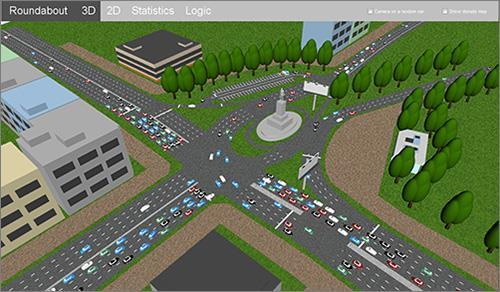
\includegraphics[width=\linewidth]{RTL.png}
\caption{Kép a \textit{Road Traffic Library}-ből \cite{anylogicpic}}
\label{fig:RTL}
\end{figure}

A szimulációkat felhasználva hőtérkép is előállítható, amely megmutatja mennyire voltak
forgalmasak az adott területek, így egyértelművé válik hol alakul ki könnyedén forgalmi dugó. Egy ilyen hőtérképet láthatunk \aref{fig:heatmp}. ábrán.

\begin{figure}[H]
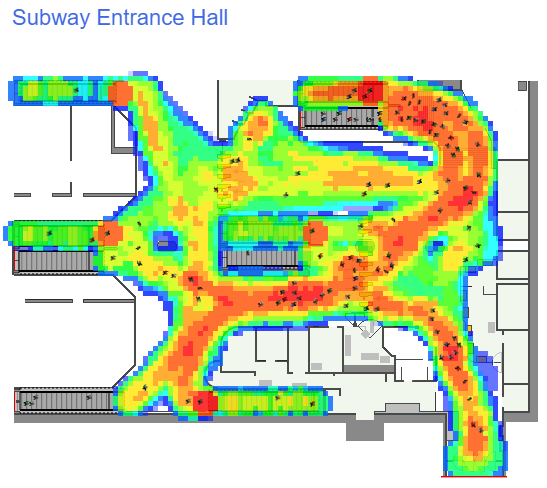
\includegraphics[width=\linewidth]{heatmap.png}
\caption{Hőtérkép egy metróállomás gyalogosforgalmáról az AnyLogic szimulációs szoftverrel\cite{heatmappic}}
\label{fig:heatmp}
\end{figure}

Lehetőség van a geoinformációs rendszerekben használt vektorgrafikus formátum, azaz \textit{shapefile} importálására is. Ezen fájl alapján a szoftver automatikusan
előállítja az úthálózatot. A szoftver bővíthető még gyalogos- és vasútforgalomra vonatkozó könyvtárakkal is.

A gyalogos könyvtár segítségével szimulálható a gyalogosforgalom sűrűsége különböző környezetekben. Ilyen környezet lehet például egy buszmegálló, vagy vasútállomás területe. Az egyes épületek
felépítése is befolyásolja a forgalom sűrűségét, a gyalogosok minden akadályt, ebbe beleértve egymást is, próbálnak elkerülni.

A vasút könyvtár segítségével egy pályaudvar vasútforgalma komplex módon szimulálható. A forgalmat befolyásolja a tehervonatok rakodási ideje, a karbantartás, üzleti folyamatok lefolyása, és sok más további esemény is.

\subsection{SUMO}

A SUMO, azaz \textit{Simulation of Urban MObility} egy ingyenes, nyílt, közlekedés-szimuláló C++-ban írt szoftver \cite{SUMO}. Az első verzió 2001-ben került kiadásra, azóta már az 1.1.0-ás verziószámnál jár. Ez a szoftver lehetőséget ad több közlekedési forma (például tömegközlekedés, gyalogosok)
modelezzésére a személygépjárművek mellett. Továbbá széles eszköztárral bír az olyanokhoz, mint útvonaltervezés, káros-anyag kibocsátás, valamint vizuális megjelenítés.
Lehetséges továbbá meglévő úthálózat importálása fájlból, valamint személyre szabott modellek használata. A SUMO nem tartalmaz semmilyen megkötést az úthálózat méretét, vagy az egyszerre szimulálható járművek számát illetően. Egy, a program által szimulált gyalogos átkelőhelyet láthatunk \aref{fig:SUMO}. ábrán.

\begin{figure}[H]
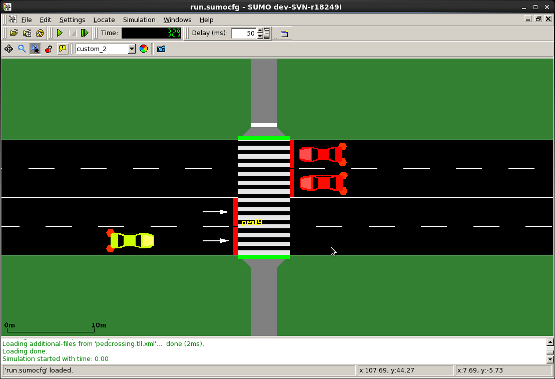
\includegraphics[width=\linewidth]{SUMO.png}
\caption{Kép a SUMO programból \cite{sumopic}}
\label{fig:SUMO}
\end{figure}

A program lehetőséget ad a szimuláció online történő kezelésére is, a \textit{TraCI}, azaz \textit{Traffic Control Interface} használatával. Ilyen esetben a SUMO tulajdonképpen egy szerver, amelyet
egy vagy több kliensen keresztül tudunk vezérelni. TCP alapú kliens/szerver architektúrát használ. 

A közlekedési lámpák viselkedését egyénileg be lehet állítani, vagy akár előre
megírt TLS programból is lehetséges importálni. Az importáláshoz számos python szkript áll rendelkezésre. Ha nem áll rendelkezésre TLS program, a SUMO képes automatikusan generálni
egyet. Ilyenkor alapértelmezett értékeket rendel minden paraméterhez amelynek értéke nem volt kapcsolókkal definiálva. Ezek közé tartoznak:
\begin{itemize}
\item \texttt{--tls.cycle.time}: lámpák váltási ideje.
\item \texttt{--tls.yellow.time}: mennyi időre sárga a lámpa, ez alapértelmezetten az utak sebességhatára alapján történik kiszámításra.
\item \texttt{--tls.minor-left.max-speed}: az útkereszteződésben balra kanyarodást megengedő sebességhatár (ha az út sebességhatára ezen érték felé esik, nem engedélyezett a balra kanyarodás.)
\item \texttt{--tls.left-green.time}: ha egyszerre kap zöldet az egyenesen haladó, és a vele szemből balra kanyarodó, ezen érték idejéig a balra kanyarodó kap elsőbbséget.
\item \texttt{--tls.allred.time}: minden zöld lámpa előtt ezen értéknek megfelelő ideig piros az összes lámpa (alapértelmezetten 0.)
\item \texttt{--tls.default-type}: \texttt{actuated} értékre állítva változó hosszúságú ideig tartanak a zöld lámpák.
\end{itemize}

A szoftver alkalmas a közlekedési lámpák teljesítményének vizsgálatára, olyan útvonal-tervezésre amely igyekszik a káros-anyag kibocsátást és a légszennyezést
minimalizálni. A gyakorlatban történt híresebb alkalmazásai tartozik például a 2006-os labdarúgó világbajnokság-, valamint a Pápa 2005-ös Kölni látogatása során a közlekedés előrejelzése.

Maga a programcsomag tartalmazza a parancssori SUMO szoftvert, a grafikus felülettel ellátott GUISIM-et, egy úthálózat importáló NETCONVERT szoftvert, úthálózat generáló NETGEN szoftvert, 
egy OD2TRIPS nevű alkalmazást amely O/D mátrix alapján generál útvonalat, számos útvonal generátort, valamint egy grafikus úthálózat-szerkesztő alkalmazást.

\Section{Meglévő térkép-adatbázisok modellje}

A \textit{Google Maps} az egyik legelterjedtebb úthálózat-vizualizálásra alkalmas szoftver. Ez egy JavaScript alapú webalkalmazás, mely a geoinformációs adatok megjelenítése
mellett valós-idejű forgalom elemzésre is képes \cite{mapsdoc}.

Ehhez az adatokat több féle forrásból állítják elő. A \textit{Base Map} program keretében rengeteg különböző forrásból
szereztek vektoradatokat a létező úthálózatokról. Később ennek a nevét \textit{Geo Data Upload}-ra váltották, viszont a lényege ugyan az maradt.
Továbbá szereznek adatokat műholdképekből, Android rendszerű okostelefonok szolgáltatásai által, valamint a nemrég bevezetett "Helyi Idegenvezetők" funkcióval, amin keresztül
bárki tölthet fel adatokat. 

A valós-idejű forgalomelemzéshez kezdetekben a helyi önkormányzatok által szolgáltatott adatokat használták, melyeket az egyes helyeken felszerelt
szenzorok segítségével gyűjtöttek be. Viszont ezek csak a legforgalmasabb utakról adtak információt, ezért később áttértek a "crowd-source" módszerhez. Ezzel a módszerrel egy
\textit{Google Maps}-et futtató okostelefon GPS adatait felhasználva ad becslést egy út forgalmasságára. Lényegében azt elemzi, mennyien küldtek GPS adatot egy adott útszakaszon azonos időben.

Az utak és más objektumok kirajzolásához a böngésző leegyszerűsített vektoradatokat kap, melyek alapján felépíti az azoknak megfelelő formákat.
Minden egyes objektumhoz tartoznak különböző metaadatok, mint például a sebességkorlát, haladási irány, út típusa (főút, stb), valamint egy név. Az objektumok JSON formában vannak
tárolva, maga a Google Maps API pedig támogatja a GeoJSON forrásból történő adatok betöltését térképekre.
Ezen információk alapján épül fel a modell amit a böngésző 2D vagy 3D formában ábrázol egy térképen.

\Section{GeoSpatial adatbázisok}

A \textit{GeoSpatial} adatbázisok adják az előbbi szolgáltatások hátterét. Ezek az adatbázisok kifejezetten a térbeli objektumokat leíró adatok tárolására, azok egyszerű lekérdezésére
vannak optimalizálva. A leggyakoribb adatok pontok, vonalak, vagy poligonok formájában fordulnak elő. 

A hagyományos adatbázisokhoz képest sokkal nagyobb teljesítményt nyújtanak
ilyen területen, valamint gyakran az ilyen típusú adatok feldolgozásához bővíteni kell azok funkcionalitását. Ennek érdekében az Open Geospatial Consortium 1997-től kezdődően
definiálta az ISO 19125 szabványt ezen funckionalitás megvalósításához, melynek második része leírja az SQL-ben történő megvalósítást is. Az OpenGIS szabvány ugyan magába
foglalja a CORBA és az OLE/COM implementációkat is, ezek nem részei az ISO szabványnak.

A szabvány többek között a következő műveleteket definiálja:
\begin{itemize}
\item térbeli számítások, azaz objektumok közöti távolság, vonalak hossza,
\item térbeli predikátumok, objektumok közötti kapcsolatokat leíró logikai lekérdezések,
\item geometriai konstruktorok, alakzatot leíró adatok alapján új geometriai elem létrehozása,
\item egy tetszőleges objektumhoz tartozó információk lekérdezése.
\end{itemize}


\Chapter{Matematikai modell részletezése}

\Section{Modell specifikálása}
A közlekedésre irányuló modell fő tulajdonságai közé kell hogy tartozzon az elegendő információ tárolása ahhoz, hogy alapvetően tudjanak a szimulált 
járművek rajta közlekedni. Ezt rengeteg féle képpen meg lehet valósítani, sokféle eleme lehet egy adott térképnek, akár minden egyes előforduló úttípusra, 
szabályra, táblára tekinthetünk úgy mint a modell egyedi része. Ez a megközelítés viszont lehetségesen túlbonyolítaná a modellt, ezáltal a procedurális generálás
nem adna annyira elfogadható úthálózatot, lehetségesen életszerűtlen helyzetek épülhetnek fel a sok elem megléte, azok elhelyeződése miatt. Sokkal inkább célszerű a 
modell részeként tekinteni a főbb építőelemeket, melyek elegendőek magához az úthálózat generálásához, valamint néhány alapvető szabályt megvalósító elemet, mint például 
a lámpás útkereszteződés, az egyirányú út, valamint a többsávos út.
\Section{A modellben használt elemek}
Matematikailag a modell egy gráfból áll, melynek csomópontjai jelölik az útkereszteződéseket, vagy két egyenes útszakasz között az összekötő részt. Az élek jelölik magát az útszakaszokat, ezeknek az éleknek pedig számos tulajdonságai lehetnek amivel különbséget teszek több elem között.
\subsection{Egyenes út}
Alapvető egyenes útszakasz, ennek lehet több paramétere is. Ennek az elemnek elsősorban tartalmaznia kell az úton létező sávok számát.
Az elem leírásához szükség van annak kezdő és végpontjára. További információt ad a modell többi részének, ha tartalmazza egy megközelítőleges égtájnak megfelelő irányt. Ebből következtetni lehet arra ha például kanyar következik, és ha igen akkor milyen irányban, csak arra van szükség rá hogy megnézzük milyen módon változik az utak hozzávetőleges iránya.

Alapvetően az út olyan szélességű, hogy elfér egymás mellett két jármű, ezért ha több sáv van csak arra kell figyelni hogy megfelelő helyen közlekedjenek az adott járművek. A gráfon való pozicíójának behatárolásához a kezdő és végpont az ő általa összekötött két csomópontot jelenti.
\subsection{Egyirányú út}
Hasonló az egyenes úthoz, viszont egyértelműen meg kell határozni a két végpont közül melyik a kiindulási, melyik a célpont. Hasonlóan az egyenes szakaszhoz, azzal a különbséggel, hogy ez az út kizárólag 1 sávos.

A gráfot tekintve itt a két összekötött csomópont között egy irányított él lesz, melynek kezdő és végpontjaként egyértelműen el kell jelölni a két pontot.
\subsection{Kanyar}
Vehető tulajdonképpen külön elemnek, de lényegében csak két egymást követő egyenes szakasz, melyek az őket összekötő elem mentén nem egyenes irányban folytatódnak. A kanyar iránya adódik az általa összekötött két egyenes útszakasz iránya által.

A gráfon kanyarnak tekinthető az olyan csomópont, melyből csak két él indul ki, ha ez a két él iránya egymástól eltérő, és nem ellentétes.
\subsection{Útkereszteződés}
Három vagy több útszakasz találkozásánál használatos elem. Tulajdonságai közé tartozhat az hogy tartalmaz-e jelzőlámpát az útkereszteződés, vagy sem.
Az útkereszteződés jellemezhető annak középpontjával, valamint az azt érintő utak halmazával.

A gráfon ez azt jelenti, hogy amennyiben egy csomópontból legalább 3 él indul ki, az egy útkereszteződés.
\begin{figure}[H]
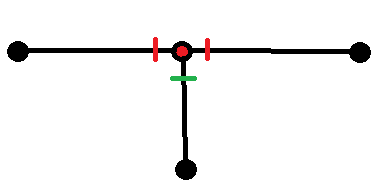
\includegraphics[width=\linewidth]{utkereszt.png}
\caption{Háromágú útkereszteződés lámpákkal}
\label{fig:xroad}
\end{figure}
\subsection{Személygépjármű}
Legalapvetőbb közlekedési jármű. Az autókról nyilván kell tartani azok jelenlegi pozícióját, mely abból adódik hogy éppen melyik élen haladnak, melyik csomópont felé, és attól milyen távolságra vannak. Minden jármű véletlenszerűen kiválasztott útvonalat kap, amin végig kell haladjon. Ezek az útvonalak a teljes gráfon egy-egy részgráfok. A jármű jellemzői közé tartozik annak sebessége, valamint a következő csomópontot elérve a várható haladási iránya, tehát előre, balra, vagy jobbra megy-e tovább. 

Tudnia kell a vele egy úton közlekedő járművekől is, azok pozíciójától függ a viselkedése. A járművek kezdetben véletlenszerű helyen kezdenek, majd ha sikeresen eljutottak a célpontjukhoz 
eltűnnek a modelből (leparkolt kocsinak tekintve). Ezen útvonal kijelölése egy véletlenszerűen kiválasztott csomóponttól indul, ahonnan véletlenszerű irányba indulunk el, majd a következő csomópontot elérve szintén új irányt választunk addig, ameddig vagy zsákutcába nem ér az autó, vagy eléri a paraméterként maximálisan kijelölt úthosszat. Szintén a paraméterezést tekintve ilyenkor új jármű jelenik meg ha jelenleg kevesebb van mint a megadott maximális érték.
\subsection{Autóbusz}
Kissé különlegesebb járműtípus, vonatkozik rá néhány további szabály. Többek között elsőbbsége van megállóból elindulva, valamint ha lehet próbál jobbra tartani,többsávos úton használhatja a külső sávot is egyenes haladásra és balra kanyarodásra. A buszmegállók között megkötött útvonalon kell haladnia, mindegyiknél pedig meg kell állnia. Ha elérte az útvonal végét megfordul, és visszafelé halad végig rajta. A szimuláció teljes ideje alatt az útvonalat követi, kezdetben az útvonal végéről elejétől indul.

Ez az útvonal a gráfot tekintve egy legmélyebb szinten elhelyezkedő véletlenszerűen választott csomópont, valamint a tőle legtávolabb lévő csomópont közötti utat jelenti. Kijelölése könnyen megoldható ezen két csomópont szüleit végigkövetve a középen lévő kiindulási pontig.
\subsection{Buszmegálló}
Autóbusznak elhelyezett megállási pont. Két csomópont közötti él felezőpontján helyezkedik el, ezért leírásához elegendő az adott élt megadni. Szükséges információ a buszmegállók közötti minimum távolság, azaz hány csomópontnak kell lennie legalább két buszmegálló között. Ezt a számot véletlenszerűen fogom meghatározni minden buszmegálló elhelyezése után újra számítva.

Ezen elem egy olyan csomópont, amelyből nem indul él, és nem is tart belé él.
\subsection{Épületek}
A gráf létrejötte után kijelölendő elemek. Az élek két oldalán helyezkednek el a házak, amelyek az alacsonyabb szinten lévő csomópontok között blokkházak, magasabb szinteknél pedig kertesházak. Az út két oldalán lévő elhelyezkedés szimmetrikus. A blokkok magassága változó.
\begin{figure}[H]
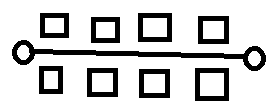
\includegraphics[width=\linewidth]{epulet.png}
\caption{Út két oldalán lévő épületek}
\label{fig:builds}
\end{figure}
\subsection{Park}
Szintén a gráf létrejötte után kerül elhelyezésre, kizárólag az utakkal teljesen közbezárt területeken. Az adott területen belülre fák kerülnek, valamint egy szökőkút.
\begin{figure}[H]
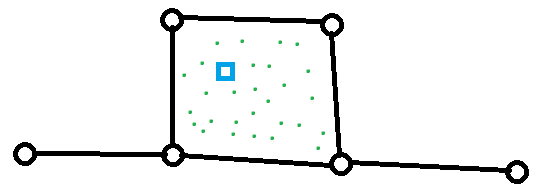
\includegraphics[width=\linewidth]{park.png}
\caption{Elkerített részen lévő park, kék négyzettel jelölve a szökőkutat, zöld pontokkal a fákat}
\label{fig:parkmodel}
\end{figure}
\subsection{Útvonal}
Ez az egy járműhőz tartozó egyedi haladási vonala az úthálózaton. Nem ugyan az, mint az útvonal éleinek kezdő és végpontja, ugyanis itt egyértelműen ki kell jelölni annak a sávnak a pontjait, amelyikben a jármű haladni fog. Útkereszteződésben ez segít a helyes irányba való kanyarodásban.
\begin{figure}[H]
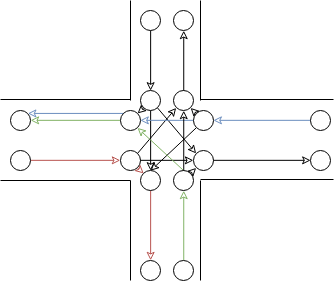
\includegraphics[width=\linewidth]{ut.png}
\caption{Egy útkereszteződésbeli útvonalakat kijelölő pontok. Példa útvonal balra kanyarodáshoz (zöld), jobbra kanyarodáshoz (piros), egyenes haladáshoz (kék).}
\label{fig:path}
\end{figure}
\subsection{Közlekedési szabályok}
Néhány alapvető közlekedési szabály amelyet a járműveknek követniük kell, általában attól az elemtől függ ahol haladnak, valamint attól amelyhez tartanak
\begin{itemize}
\item Egyirányú útra csakis a kijelölt útirányban hajthatnak rá a járművek
\item Ha az út több sávot tartalmaz, a külső sáv csak jobbra kanyarodásra alkalmas, a belső sáv balra kanyarodásra, illetve egyenes haladásra
\item Ha az útmenti buszmegállóból elindulni készül a busz, a többi járműnek elsőbbséget kell neki adnia
\item Jelzőlámpával ellátott útkereszteződésbe nem hajthat be ha a lámpa piros, ha aközben vált hogy benne van akkor még áthaladhat
\end{itemize}
\Section{A modell kritériumai}
\subsection{Generálási szempont}
Magának az úthálózatnak a generálására vonatkozóan a következők a célok:
\begin{itemize}
\item Viszonylag kevés elemből álljon össze a generált úthálózat
\item Ne legyen életszerűtlen az összeállított úthálózat
\item Tartalmazza az alapvető közlekedési helyzetek szimulálására szükséges elemeket
\item Vizuálisan emlékeztessen egy átlagos városra
\item Bizonyos mértékig paraméterezhető legyen, főleg a méreteket érintve
\end{itemize}
\subsubsection{Elemek száma}
Az említett viszonylag kevés elem, vagy pontosabban kevés különbözű típusú elem azt jelentené, hogy ne legyenek túl specifikusak az elemek, hanem akár könnyedén egyik elem bővítésével elő lehessen állítani egy másikat. Ilyen például a modellben az egyenes szakasz, melyből kis változtatással előáll az egyirányú út.
\subsubsection{Életszerű úthálózat}
Röviden annyit tesz, hogy nem tartalmaz olyan területeket ahol össze van szűkítve kis területen rengeteg út. Tehát legyen minimális hely kihagyva az utak között az épületeknek. Életszerűtlennek tekinthető továbbá az is, ha egy útkereszteződésből rengeteg út indul ki, azaz 5-6 avagy annál több. Ezért a modellben az útkereszteződés maximálisan 4 utat köthet össze.
\subsubsection{Közlekedési helyzetek}
Legyen benne jelzőlámpával ellátott útkereszteződés, többsávos út, egyirányú út, valamint buszmegálló. Ezek az elemek szükségesek minden esetben, hogy a szimuláción meg lehessen jeleníteni a lámpák működését, a többsávos utak eseten a járművek sávválasztását és tartását, egyirányú út irányának a betartását, és buszmegállónál a busz megállását, neki járó elsőbbség megadását.
\subsubsection{Átlagos város képe}
Átlagos városra hasonlít akkor, ha a központtól kifelé haladva ritkul az úthálózat, valamint a többsávos utak az előreláthatólag forgalmasabb helyeken vannak elhelyezve. Ennek érdekében a modellben elhelyezett csomópontok átlagosan kevesebb élt indítanak magukból, minél távolabb vannak a gráf kiindulási pontjától, azaz a középponttól.
\subsubsection{Paraméterezés}
Ki lehessen jelölni hogy a generálás meddig tartson, azaz hány csomópontot terjesszen ki. 
\subsection{Szimulációs szempont}
A már legenerált úthálózaton a szimulációra tekintve ezek a célok:
\begin{itemize}
\item A járművek kövessék a modellben definiált alapvető szabályokat
\item A szimuláció bizonyos mértékben paraméterezhető legyen, főleg a járművek számát illetően
\item Reagáljanak egymásra a járművek
\item Ne legyen életszerűtlen a járművek viselkedése
\item Teljesítmény szempontjából elfogadható legyen egy adott méretig
\end{itemize}
\subsubsection{Szabályok}
A már előbbiekben leírt szabályoknak megfelelően közlekedjenek a járművek, haladási útukat azok alapján válasszák meg.
\subsubsection{Paraméterezés}
Meg lehessen adni mennyi jármű legyen maximálisan egyidőben az úthálózaton, külön értve a buszokat ettől. Továbbá az is megadható legyen milyen gyakorisággal jelenik meg személygépjármű, és mekkora lehessen a neki kijelölt útvonal maximális hossza csomópontokban mérve.
\subsubsection{Reagálás}
Ha egy jármű közelít egy másik felé kezdjen lassítani. Ez a lassítás függjön a távolság mértékétől, ha elég közel kerül hozzá teljesen álljon meg. Csak akkor induljon el egy jármű, ha haladási útját nem állja el másik jármű. Közúti baleset, azaz ütközés esetén a két érintett jármű kis idő után tűnjön el, ezzel szemléltetve az elszámolás, elvontatás folyamatát.
\subsubsection{Életszerű viselkedés}
A járművek tartsák az út vonalát, ne térjenek át a szembe sávba. Gyorsítás és lassítás viszonylag realisztikusan történjen, ne pedig hirtelen. Kanyarodás előtt igyekezzenek lelassítani, kanyart pedig végig lassan bevenni.
\subsubsection{Teljesítmény}
A szimuláció mérete mind az úthálózat csomópontjait, mind az egyszerre megjelenő autók számát értem. Abban az esetben ha ezek az értékek nem kimagaslóan nagyok, a szimulációnak lényegesebb teljesítményromlás nélkül kell futnia.
\Chapter{Generálás}

\Section{Úthálózat Generálása}

Maga a generáló algoritmus megalkotásakor első lépésben a működésre vonatkozó elvárásokat vizsgáltam. Az úthálózatnak a középponttól kifelé haladva ritkulnia kell, ezzel közelítve egy 
valódi város elrendezését. A paraméterezéssel kapcsolatos elvárásokat könnyen meg lehet valósítani. Egy gráfként képzelhető el az úthálózat, melynek csomópontjai jelölik az egyes útelemek 
elejét, élei pedig azoknak a tartományát. A gráf 0. szintjét jelöltem el a hálózat középpontjának. Ebből mindig 4 irányba indulnak ki élek. Mivel az egy csomópontból kiinduló maximális élek számának 4-et választottam,
 ez garantálja hogy a középpontnak kijelölt ponttól minden irányba nagyjából egyenletes mértékben terjedjen az úthálózat. Minden további csomópont generálódásakor kapja meg 
annak értékét, hogy mennyi irányba indulnak belőle élek. A generálás folyamatát \aref{fig:flowchart}. ábrán láthatjuk.

\begin{figure}[H]
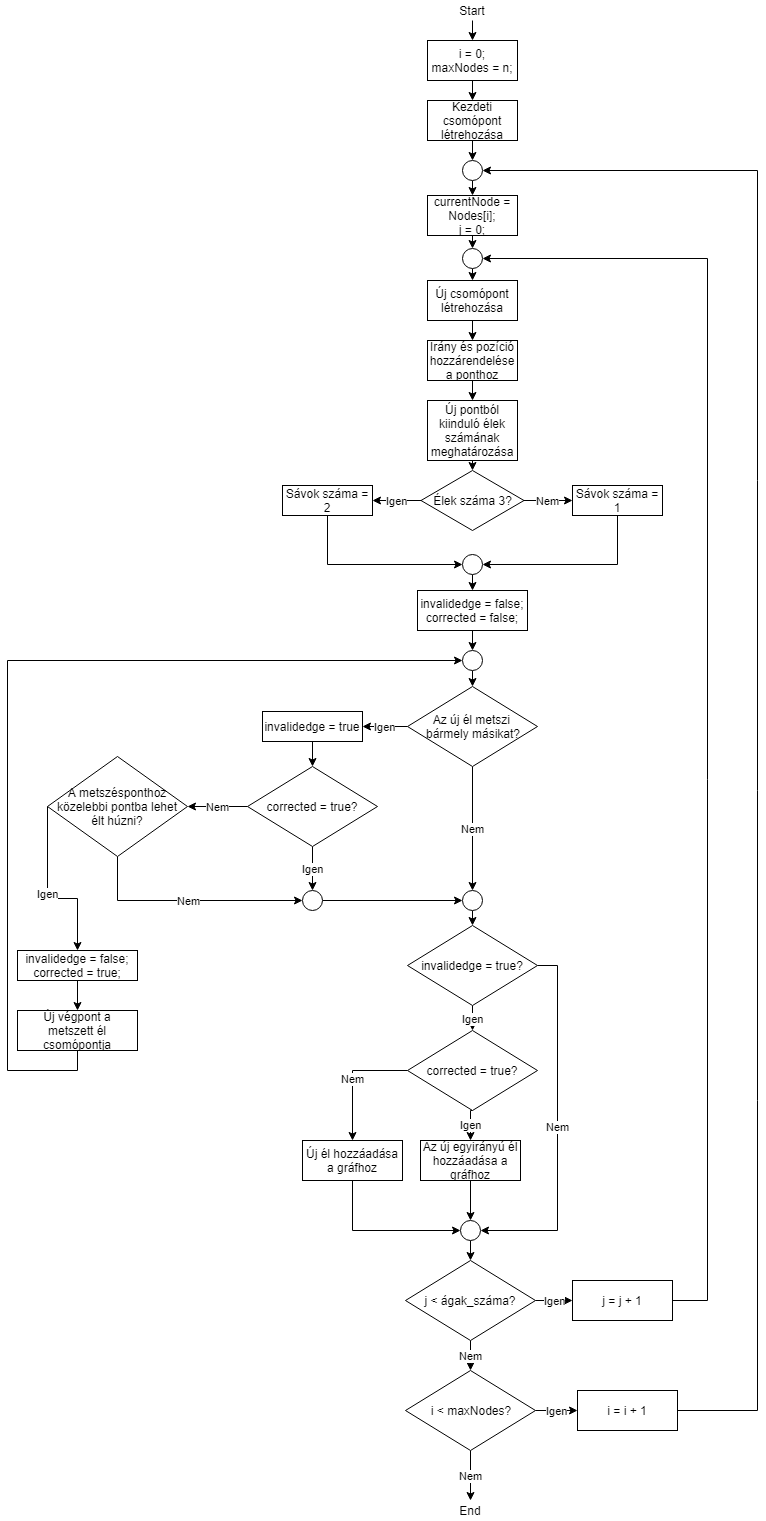
\includegraphics[keepaspectratio,scale=0.45]{folyamat.png}
\caption{A generálás lépéseinek egyszerűsített folyamatábrája}
\label{fig:flowchart}
\end{figure}

\subsection{Generáló algoritmus}

A csomópontok generálása a következő lépésekben történik.
\begin{enumerate}
\item A kiválasztott csomópont kap egy véletlenszerű irányt, észak, dél, kelet, vagy nyugat értékében.
\item Ha a kapott érték megegyezik azzal az iránnyal amerre a csomópont szülője van, vagy már indult arra belőle él, újat kap.
\item A kiválasztott iránynak megfelelő véletlen generált $X$ és $Y$ koordinátákat kap.
\item A kapott koordinátákból alkotott csomópont felkerül a gráfra.
\item Ha a jelenlegi csomópontból még kell éleket indítani, akkor kezdődik előröl.
\end{enumerate}
Az előbbiekben említett $X$ és $Y$ koordinátát kissé pontosítanám. Ha a csomópontot nyugat vagy kelet irányba generáljuk, az $X$ koordináta értéke a jelenlegi pont $X$ koordinátája, hozzáadva egy
előre definiált értékek közötti véletlen számot. Az $Y$ koordináta ilyenkor egy minimális eltérés az út fekvésében, hasonlóan generálódik, de lényegesen kisebb értékű véletlen számot kap. Ez
tulajdonképpen a valóságban is látható "tökéletlenségekre" vezethető vissza, ugyanis a legtöbb esetben ott sem teljesen merőleges egymásra két út. Az észak és dél irányba induló pontok 
esetén ugyan ez az eljárás, csak a két koordináta szerepe felcserélődik.
Fontos viszont az is, hogy a középponttól távolodva átlagosan kevesebb elágazása legyen egy csomópontnak, ezért ehhez felhasználható annak gráfbeli szintje. Minden csomópontról eltárolódik 
annak szintje (szülő szintje + 1), ami befolyásolja az elágazások számát. Egy másik probléma az, hogy az így generált élek gyakran metszhetik egymást, amely az aluljárók és a hídak hiányában 
itt nem megengedett, ezért utolsó lépésnek ellenőrizni kell hogy az új él metszi-e bármely meglévő élek közül akár az egyiket is, és ha igen akkor nem kerülhet fel a gráfra. Az él viszont hozzáadható 
az eredetileg kijelölt csomóponthoz legközelebbi csomóponttal történő helyettesítéssel, feltéve ha így nem történik létező út metszése.
A buszmegállók elhelyezésével kapcsolatban a következő feltételeket
adtam.
\begin{itemize}
\item A legcélszerűbb a hálózat két, egymástól távol lévő, a gráf mélyebb szintjein elhelyezkedő pont közötti út létrehozása.
\item Az útvonalnak érintenie kell a középpontot, a gráf 0. szintjét.
\item Lehető legkevesebbszer érintse többször ugyan azt a csomópontot.
\end{itemize}
Ennek érdekében először kijelölöm az út egyik végét, mint megállót. Ezek után keresek egy utat a gráf 0. szintjéhez, melyen legfeljebb minden második csomópontot kijelölöm megállónak. A középpont 
elérése után kijelölöm a második végpontot, mely a középponttól az eddigi iránynak ellentétesen, a gráf mélyebb szintjei közül kell lennie. Az ehhez a középpontból vezető úton, az utóbbihoz hasonló 
eljárással kijelölök megállókat. Az utak sávszámának meghatározására a gráfbeli mélységüket használom. A magasabb szinten lévő élek nagyobb valószínűséggel lesznek többsávosak. Ez a generálás végén választódik
ki. Az egyirányú utak kijelölése is a folyamat legvégén történik. Ennek az oka magából az utak jellegéből adódik, ugyanis egyirányú út nem végződhet zsákutcában, és nem is zárhatja el a hálózat egy részét a többi elől. Éppen ezért egy olyan részgráfot kell találni amely Hamilton-kört alkot, amelyen egy részgráfot már nyugodtan egyirányúvá lehet tenni.

\subsection{Az egyirányú út}

Egy könnyű módszer annak megoldására, hogy mely utak lehetnek egyirányúak az lenne, ha a generálás során egymást metszett utakból kialakult éleket jelölöm el egyirányúnak. Ezek az élek ugyanis biztos hogy egy létező Hamilton-út részei, mivel az eredetileg fagráfnak megfelelő úthálózat bármely két csomópontja közé húzott él Hamilton-utat ad.

\Section{Alapelemek megjelenítése HTML Canvas segítségével}

\subsection{Fejlesztői környezet felállítása}

Az algoritmus működését, eredményét egy \textit{HTML Canvas} objektumon szemléltetem. Magát a kódot \textit{JavaScript}-ben írtam, annak ECMAScript 6-os verziójában. Fejlesztői környezetnek A \textit{JetBrains} által készített \textit{WebStorm} fejlesztőkörnyzetet használtam. Először
létrehoztam egy HTML fájlt, ahol a \texttt{body} tag-en belül elhelyeztem a canvas elemet. Erre az elemre JavaScriptből a HTML-ben megadott id-je alapján lehet hivatkozni. Ezután létrehoztam egy JavaScript fájlt, melyben egy \texttt{(document).ready()} szintaktikában 
elhelyezett függvényhívással indítom a generálást. A \texttt{(document).ready()} a \textit{jQuery} függvénykönyvtárnak része. Azért szükséges ebben az esetben, mert ameddig a html fájl nem töltött be teljesen, a script nem futtatható mert a canvas elemre nem létezne 
semmilyen referencia. Ez a részlet biztosítja hogy csak akkor kezdődjön a script futtatása, ha a HTML documentum teljesen betöltött. A js fájlban globálisan eltárolom egy változóba a canvasre mutató referenciát, majd egy másik váltózóba lekérem ennek a kontextusát.

\subsection{Létrehozott osztályok}

\subsubsection{Node}

A gráfon egy csomópontot leíró objektumot \texttt{Node}-ként definiáltam. Ez egy konstruktort tartalmaz, amely beállítja az osztály 6 adattagjának értéket. Ezek az adattagok a következőek:
\begin{itemize}
\item \texttt{x}: a csomópont $X$ koordinátája,
\item \texttt{y}: a csomópont $Y$ koordinátája,
\item \texttt{branches}: megadja, hogy hányfelé kell tovább ágaztatni a csomópontot,
\item \texttt{level}: azt mutatja, hogy a gráf hanyadik szintjén helyezkedik el a csomópont,
\item \texttt{connectedFrom}: milyen irányból lett kiterjesztve a csomópont,
\item \texttt{parentNodeIndex}: a gráfban lévő csomópontokat tartalmazó vektoron belül ezen csomópont szülőjének indexe.
\end{itemize}

\subsubsection{Edge}

Az \texttt{Edge} a gráfon egy él leírására szolgáló objektum típusát definiálja. Egy konstruktort tartalmaz, amely inicializálja 4 adattagját. Ezek az alábbiak:
\begin{itemize}
\item \texttt{from}: Az a csomópont, ahonnan az él kezdődik
\item \texttt{to}: Az a csomópont, amiben az él végződik
\item \texttt{lanes}: Az él által jelölt úton hány sáv van
\item \texttt{oneway}: Logikai változó, az út egyirányú-e vagy sem
\end{itemize}

\subsubsection{Graph}

Magát a gráfot leíró objektum, mely tartalmaz 2 függvényt annak canvas-on történő kirajzolására. Paraméter nélküli konstruktora 2 adattagját inicializálja üres értékkel. Adattagjai és függvényei a következők.
\begin{itemize}
\item \texttt{Nodes}: a csomópontokat tartalmazó vektor,
\item \texttt{Edges}: az éleket tartalmazó vektor,
\item \texttt{drawAllNodes}: függvény, mely végig iterál a Nodes vektoron, és mindegyik elemére meghívja a kirajzoló függvényt,
\item \texttt{drawAllEdges}: függvény, végig iterál az \texttt{Edges} vektoron, egyirányú út esetén nyilat rajzol, ellenkező esetben egyenes vonalat.
\end{itemize}

\subsection{Segédfüggvények}

\subsubsection{intersects}

Az \texttt{intersects} függvény arra szolgál, hogy kiszámítsa két él metszi-e egymást. Ehhez két paramétert vár, \texttt{edge1} és \texttt{edge2} néven. Visszatérési értéke logikai típusú.
Működésében a két szakaszból egyeneseket képez, majd ezek alapján az \texttt{X = v1 + lambda * d1}, \texttt{X = v2 + gamma * d2} egyenletrendszer mátrixának kiszámolja a determinánsát. Ha ez 0, a két szakasz nem metszi egymást.
Ellenkező esetben megnézi az egyenletrendszerben szereplő \texttt{gamma} és \texttt{lambda} értékeket, azaz a két egyenes mentén az irányvektor hányszorosát kell venni hogy elérkezzünk a ponthoz. Ha ez nem 0 és 1 közé esik, a metszéspont nincs a szakaszon belül.
\begin{cpp}
function intersects(edge1,edge2) {
    let det, gamma, lambda;
    det = (edge1.to.x - edge1.from.x) * (edge2.to.y - edge2.from.y) - 
    (edge2.to.x - edge2.from.x) * (edge1.to.y - edge1.from.y);
    if (det === 0) {
        return false;
    } else {
        lambda = ((edge2.to.y - edge2.from.y) * (edge2.to.x - edge1.from.x)
         + (edge2.from.x - edge2.to.x) * (edge2.to.y - edge1.from.y)) / det;
        gamma = ((edge1.from.y - edge1.to.y) * (edge2.to.x - edge1.from.x)
         + (edge1.to.x - edge1.from.x) * (edge2.to.y - edge1.from.y)) / det;
        return (0 < lambda && lambda < 1) && (0 < gamma && gamma < 1);
    }
}
\end{cpp}

\subsubsection{distance}

A \texttt{distance} két csomópont közötti távolság kiszámítására szolgáló függvény. Ehhez a két vektor által meghatározott szakasz hosszát számolja ki pitagorasz tétellel. Ezzel az eredménnyel tér vissza.

\subsubsection{maxBranchesReached}

A \texttt{maxBranchesReached} függvénnyel megmondható hogy egy adott csomópontba már lett-e 4 él húzva. A függvény paramétereiként megkapja a keresett csomópontot, a gráfot, és a jelenleg kiterjesztés alatt álló csomópont gráfbeli indexét. Amennyiben a gráfban megtalált csomópont \texttt{branches} értéke kisebb mint 3, akkor növeli 1-el és hamis értékkel tér vissza, azaz még nem volt 4 él húzva. Ellenkező esetben igaz értéket ad.

\subsubsection{getBranchCount}

A \texttt{getBranchCount} függvény egy egész számot kap paraméterként, mely egy csomópont gráfbeli mélységére utal. Ez alapján a szám szerint visszaadja hogy mennyi irányba ágazzon el az adott csomópont. Első szinten 80\% az esélye hogy 4 irányban ágazik el, ez szintenként 20\%-al csökken. Ha nem 4 irányban ágazik el, véletlenszerűen generált számot ad vissza 0 és 2 között, mivel a csomópont szülőjéhez vezető élt ilyenkor nem számoljuk.

\subsubsection{findMaxLevelNodes}

A \texttt{findMaxLevelNodes} a gráf legmélyebb szintjén lévő csomópontok megtalálására szolgáló függvény. Paraméterként megkapja a gráfot. Első lépésben beállítja a max értéket a gráf első csomópontjának szintjére, és inicializálja a maximális mélységben elhelyezkedő csomópontok vektorát. Ezután maximum kereséssel beállítja max értéket. Majd a gráf \texttt{Nodes} vektorán végig iterálva hozzáadja az ezen max értéknek megfelelő mélységű csomópontokat az eredmény vektorhoz. Végül ezzel a vektorral tér vissza.

\subsubsection{DrawBStops}

A \texttt{DrawBStops} a buszmegálló rajzolására használt függvény. Egy csomópontot kap paraméterként. A kontextust felhasználva felrajzolja a canvasra egy zöld négyzet formájában. Visszatérési értéke nincs.

\subsubsection{makeBusStops}

A \texttt{makeBusStops} függvény szolgál a buszmegállók elhelyezésére. Egyelőre csak a hozzávetőleges helyüket jelöli, nem az él közepére teszi a helyüket, hanem a csomópontokra. Paraméterként megkapja a gráfot. Előszőr meghívja a findMaxLevelNodes függvényt, ebből a kapott értéket eltárolja egy változóba. 

Kijelöl az útvonal kezdetének az előbb kapott vektorból egy véletlenszerű elemet. Ezt felrajzolja a \texttt{DrawBStops} függvénnyel. Ezután végig iterál a maximum mélységű tömbökön, maximum keresést végezve a kiindulási ponttól mért távolságot illetően. Ehhez a \texttt{distance} függvényt használja. Ha megvan a végpont azt is felrajzolja. 
Ezután elindul a kiindulási ponttól, sorra véve a csomópontok szüleit. Minden buszmegálló kirajzolása után kap egy véletlen értéket, amely megmondja hogy hány csomópont után kell rajzolnia mégegyet. Ha eljutott a gráf kezdőpontjáig megcsinálja ugyan ezt az út végpontjától is. Visszatérési értéke nincs.

\subsubsection{drawCanvasNode}

Egy paraméterként megkapott csomópont koordinátáinak megfelelő helyre négyzetet rajzol a canvasre.

\subsubsection{drawCanvasEdge}

Egy élt kap meg paraméterként, melynek kezdő és végpontjai között egyenes vonalat húz a vászonra.

\subsection{A generáló függvény}

A generálás kódjának fő része ebben a függvényben van. Ez egy paraméter nélküli függvény, visszatérési érték nélkül. A következőkben vázolom a működését. 

Először inicializálja a gráfot az osztály példányosításával, majd kijelöli a kezdő csomópontot, annak paramétereit beállítva fix értékekre, tehát 4 elágazású lesz, az $(1000, 500)$ koordinátákon. 

Ezután egy ciklussal végig iterál a csomópontokat tároló vektoron, minden csomóponton kezdetben megadja a \texttt{connectedFrom} értéket, tehát hogy az adott csomópont melyik irányból lett kiterjesztve. 

Ha ez megvan, újabb ciklus kezdődik, mely a csomópont elágazásait terjeszti ki egyesével. Ezen belül megkapja minden iterációban a kiterjesztés irányát, az új csomópont elágazásainak számát a getBranchCount függvénnyel, valamint az új élen lévő sávok száma is kiszámítódik. Ilyenkor már létezik az új él és csomópont mint objektum, következő lépésben megnézi hogy az új él metszi-e bármely meglévő élt. Ez egy szimpla iteráció az éleket tartalmazó vektoron, az intersects függvény segítségével eldönti hogy történt-e metszés.

Amennyiben volt metszés, de az élt be lehetett húzni a metszett élnek a metszésponthoz közelebb álló csomópontjához, az új él megmarad, és egyirányú lesz, a csomópontot pedig elvetjük. Ha nem lehetett behúzni, vagy még így is történt metszés, akkor mindkettőt elvetjük. Ezen vizsgálat után az új él és csomópont amennyiben valamelyik is alkalmas maradt, hozzáadásra kerülnek a gráfbeli vektorhoz.

Miután a kellő mennyiségű csomópont ki lett terjesztve, a függvény meghívja a gráfon belüli drawAllNodes és drawAllEdges függvényeket, majd végül a makeBusStops függvényt. Ezzel kész a generálás, az elemek felkerültek a canvasre (\ref{fig:graph}. ábra).

\begin{figure}[H]
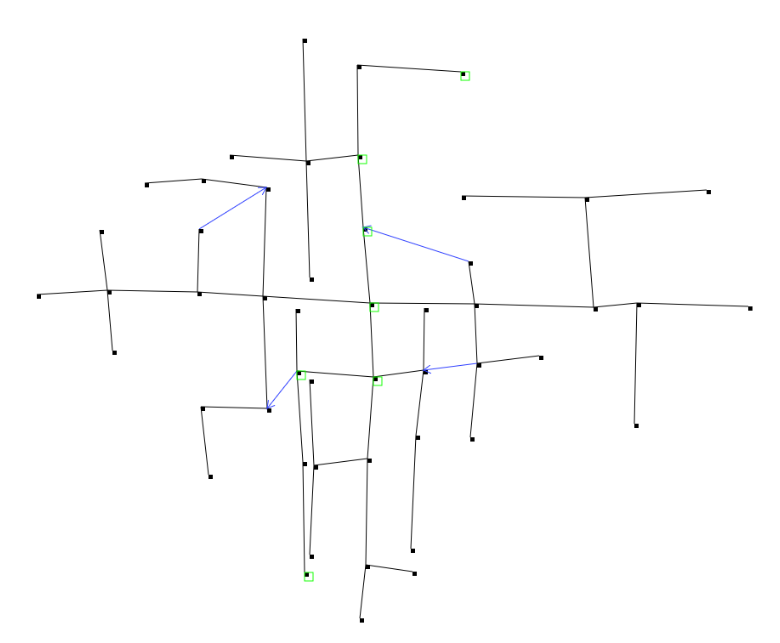
\includegraphics[width=\linewidth]{graph.png}
\caption{Kép a generáló algoritmus eddigi eredményéről}
\label{fig:graph}
\end{figure}

\Section{Az algoritmus implementálása Unity-ben}

Mivel a szimulációt a \textit{Unity Engine}-el fogom elkészíteni, első lépésben az előbbi JavaScript implementációt ki kell bővíteni. Ez főleg a kirajzoló függvények átírását fogja jelenteni, amelyben 2D canvas helyett most már 3D-s megjelenítésben kell gondolkozni, de ezen kívül a C\# programnyelvre való áttérés miatt lehetnek még minimális változtatások.

\begin{figure}[H]
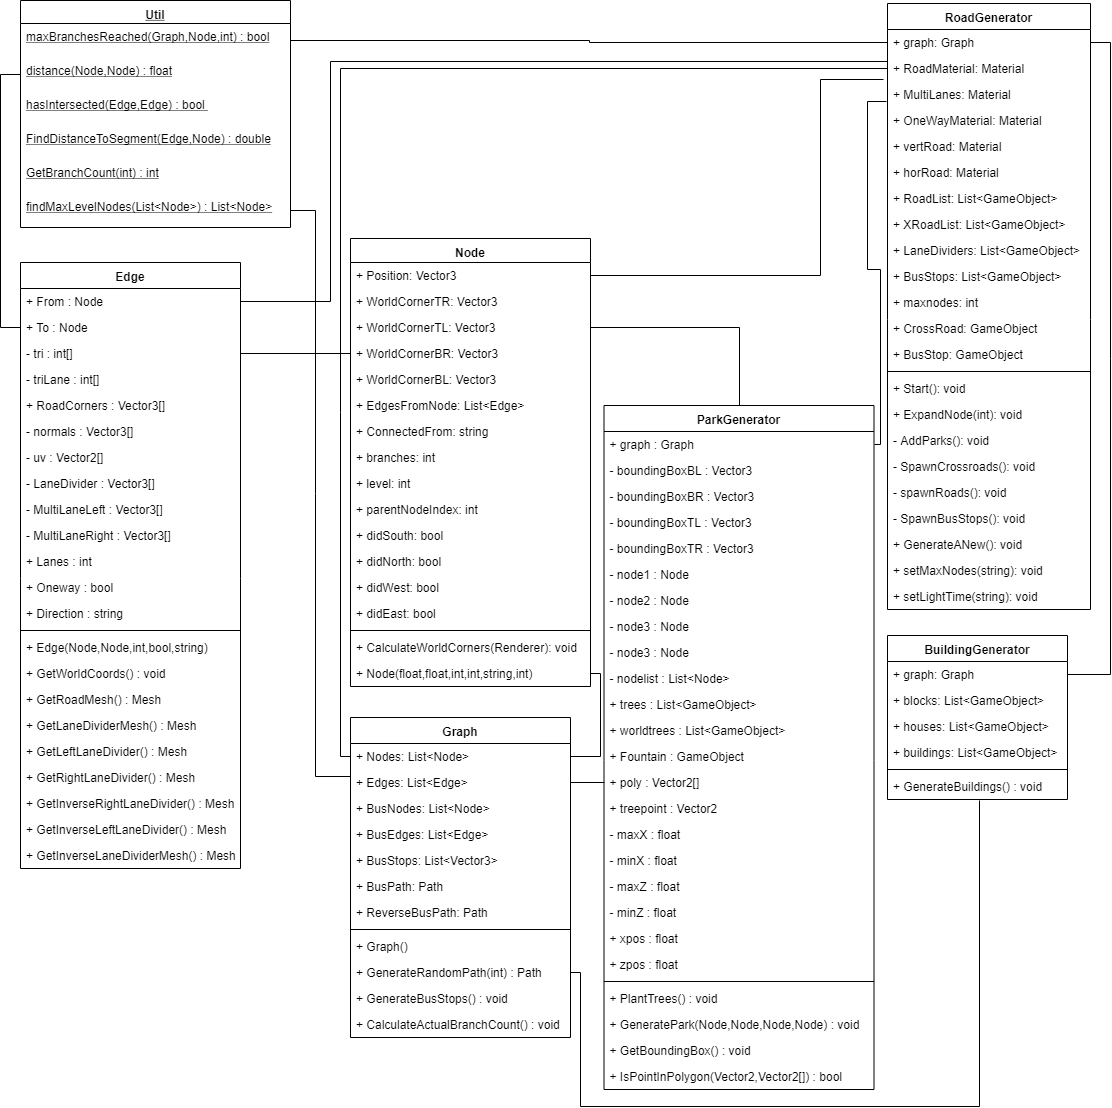
\includegraphics[scale=0.45,keepaspectratio]{generateuml.png}
\caption{A generálásban résztvevő osztályok UML osztálydiagramja}
\label{fig:genuml}
\end{figure}

\subsection{Osztályok}

A generáláshoz definiált osztályok hierarchiáját \aref{fig:genum1}. ábrán láthatjuk.

\subsubsection{Util}

Létrehoztam egy \texttt{Util} nevű statikus osztályt, melynek fő célja az lenne hogy külön osztályba összegyűjti az összes használt matematikai Segédfüggvényt. Ebbe az osztályba került bele a maxBranchesReached, a distance, az \texttt{intersects} mostmár \texttt{hasIntersected} néven, a \texttt{getBranchCount}, valamint a \texttt{findMaxLevelNodes} függvények. 

Továbbá, bővült egy újab fügvénnyel, a \texttt{FindDistanceToSegment}-el. Ez a függvény paraméterként egy élt és egy csomópontot vár. Visszatérési értékként a csomópont és a szakasz közötti legrövidebb távolságot adja.

\subsubsection{Node}

Ez az osztály az eredeti implementációhoz nagy mértékben hasonló. Egy lényeges különbség, hogy a csomópont pozícióját egy \texttt{Vector3} típusú adattagban tárolom. Ez a típus 3 \textit{float} típusú koordinátát tárol, az $x$, $y$ és $z$ koordinátákat.

Hozzáadtam valamint 5 új adattagot, amelyek közül 4 a csomóponthoz tartozó objektum négy sarkát jelőlik. Ezek az adattagok \texttt{Vector3} típusúak, kiszámításukra az osztályon belül elhelyeztem egy \texttt{CalculateWorldCorners} függvényt, melynek paraméterül meg kell adni a létező csomópont objektum Renderer komponensét.

Az ötödik új adattag egy \texttt{Edge} lista, mely a csomópontból kiinduló éleket tartalmazza, nem beleértve az ide érkezőket.

A \texttt{CalculateWorldCorners} függvény a következő képpen használja fel a renderert: a renderer objektum képes visszaadni a hozzá tartozó 3D mesht behatároló téglatestet. Ennek a téglatestnek lekérdezhető a maximum és minimum értéke, mely rendszerint a jobb felső és a bal alsó sarkát adja vissza. Ezen két pont tudatában kiszámítható a maradék két sarok is, a koordináták vegyes felhasználásával.
\begin{cpp}
public void CalculateWorldCorners (Renderer renderer)
        {
            WorldCornerTR = renderer.bounds.max;
            WorldCornerTL = new Vector3(renderer.bounds.min.x, 
            0.1f, renderer.bounds.max.z);
            WorldCornerBL = renderer.bounds.min;
            WorldCornerBR = new Vector3(renderer.bounds.max.x,
            0.1f, renderer.bounds.min.z);
        }
\end{cpp}

\subsubsection{Edge}

Ez az osztály esett át a legnagyobb átalakításon, ugyanis az utat ábrázoló mesht dinamikusan kell kirajzolni, amelyhez először el kell végezni néhány számítást.

A konstruktora változatlan maradt, viszont az osztály rengeteg adattaggal bővült. Először is a RoadCorners Vector3 típusú tömbbel, amely az útszakasz négy sarkának koordinátáit tárolja. A mesh megalkotásához szükséges a poligont alkotó háromszögek megadása, erre létrehoztam egy egész típusú tri tömböt.

Szintén hasonlóan, az úton jelen lévő felezővonalak, sávelválasztó vonalak jelölésére is szükség van egy objektumra. A felezővonal sarkait a \texttt{LaneDivider} tömbbe, a bal és jobb oldali sávelválasztó sarkait pedig a \texttt{MultiLaneLeft} és \texttt{MultiLaneRight} \texttt{Vector3} típusú tömbben tárolom. Ezeknek a válaszvonalaknak külön háromszög tömböt is deklaráltam \texttt{triLane} néven.

A poligonhálóhoz szükséges még normálvektorokat tartalmazó, illetve \textit{uv} tömböket is bevezettem.

Az osztály új metódusokkal bővült, ezek közül első a \texttt{GetWorldCoords} void típusú paraméter nélküli metódus. Ez a metódus annak függvényében, hogy a Direction adattagban milyen irány van megadva, kiszámolja az általa összekötött csomópontok sarkai alapján az útszakasz sarkainak koordinátáit.
\begin{cpp}
case "north":
                    RoadCorners[0] = From.WorldCornerTL;
                    RoadCorners[1] = From.WorldCornerTR;
                    RoadCorners[2] = To.WorldCornerBL;
                    RoadCorners[3] = To.WorldCornerBR;
                    LaneDivider[0] = ((RoadCorners[0] + 
                    RoadCorners[1]) / 2) + Vector3.up * 5;
                    LaneDivider[1] = ((RoadCorners[0] + 
                    RoadCorners[1]) / 2) + Vector3.up * 10;
                    LaneDivider[2] = ((RoadCorners[2] +
                     RoadCorners[3]) / 2) + Vector3.up * 5;
                    LaneDivider[3] = ((RoadCorners[2] + 
                    RoadCorners[3]) / 2) + Vector3.up * 10;
                    if (Lanes == 2)
                    {
                        MultiLaneLeft[0] = ((RoadCorners[0] + 
                        Vector3.up * 5) + LaneDivider[0]) / 2;
                        MultiLaneLeft[1] = ((RoadCorners[0] + 
                        Vector3.up * 10) + LaneDivider[1]) / 2;
                        MultiLaneLeft[2] = ((RoadCorners[2] + 
                        Vector3.up * 5) + LaneDivider[2]) / 2;
                        MultiLaneLeft[3] = ((RoadCorners[2] +
                        Vector3.up * 10) + LaneDivider[3]) / 2;
                        MultiLaneRight[0] = ((RoadCorners[1] + 
                        Vector3.up * 5) + LaneDivider[0]) / 2;
                        MultiLaneRight[1] = ((RoadCorners[1] + 
                        Vector3.up * 10) + LaneDivider[1]) / 2;
                        MultiLaneRight[2] = ((RoadCorners[3] + 
                        Vector3.up * 5) + LaneDivider[2]) / 2;
                        MultiLaneRight[3] = ((RoadCorners[3] + 
                        Vector3.up * 10) + LaneDivider[3]) / 2;
                    }
                    break;
\end{cpp}
Példa esetként, ha észak felé tart az út, akkor a kiindulási pont bal és jobb felső, a célpont bal és jobb alsó koordinátáira lesz szükség.

Ha az út két sávos, ezen sarkok alapján kiszámolja a felező- és sávelválasztó vonalak sarkait. Ezek megjelenésével nem kell foglalkozni, csak jelző értékkel rendelkeznek a járművek számára, ezért az útszakasz felett foglalnak helyet, egész pontosan 5 egységnyi értékkel felette.

Ezek után beállítja a tri és triLane értékeit, azaz hogy a háromszögek megalkotásához milyen sorrendbe járja be az adott pontokat.


A \texttt{GetRoadMesh} metódus maga az utat reprezentáló Mesh objektummal tér vissza. Paraméter nélküli metódus. Első lépésben meghívja a \texttt{GetWorldCoords} függvényt, ezzel beállítva az út sarkainak értéket. Majd létrehoz egy új \texttt{Mesh} objektumot, melynek csúcsait beállítja az előbb kiszámolt pontokra, háromszögek értéket pedig a tri tömbre. A normálvektorok itt nem kapnak nagy jelentőséget, $z$ tengely szerinti negatív egyenes értéket adtam nekik. Az $(u, v)$ koordinátákat szimplán a \textit{mesh} négy sarkának jelöltem el.
\begin{cpp}
public Mesh GetRoadMesh()
        {
            GetWorldCoords();
            Mesh mesh = new Mesh();
            mesh.vertices = RoadCorners;
            mesh.triangles = tri;
            normals[0] = -Vector3.forward;
            normals[1] = -Vector3.forward;
            normals[2] = -Vector3.forward;
            normals[3] = -Vector3.forward;
            mesh.normals = normals;
            uv[0] = new Vector2(0, 0);
            uv[1] = new Vector2(1, 0);
            uv[2] = new Vector2(0, 1);
            uv[3] = new Vector2(1, 1);
            mesh.uv = uv;
            return mesh;
        }
\end{cpp}
A \texttt{GetLaneDividerMesh}, \texttt{GetLeftLaneDivider}, valamint a \texttt{GetRightLaneDivider} metódusok az előbbivel hasonló módon funkcionálnak, csak a csúcsok halmaza változik.

Ám ezekkel a vonalakkal kapcsolatban szükség volt létrehoznom három Inverse metódust is, a \texttt{GetInverseLeftLaneDivider}, \texttt{GetInverseRightLaneDivider}, és a \texttt{GetInverseLaneDividerMesh} függvényeket. Erre az a magyarázat, hogy ezek alapvetően síkok, azaz a hátlapjaik nem láthatóak. 

Bár a \textit{Unity} tartalmaz megoldást ütközők konvexé alakítására, ez ebben az esetben nem mindig működik, mert gyakran a válaszvonal négy csúcsai koplanáris pontok. Ezért a következő megoldást választottam: a létrehozott síkokkal megegyező pozícióban létrehozom a síkok ellentétes irányba néző változatát. Ezt a feladatot látják el ezek az inverse metódusok, melyek az adott háromszög tömböt visszafelé járják be.

\subsubsection{Graph}

A gráfot leíró osztály bővült néhány új adattaggal. 

Külön \texttt{Node} és \texttt{Edge} listában tartalmazza mostmár a buszok útvonalát leíró csomópontokat és éleket. A buszmegállok koordinátái tárolására egy \texttt{Vector3} típusú listát is bevezettem.

Továbbá ebben az osztályban tárolom a buszok számára kirendelt útvonalat is, melyet egy \texttt{Path} nevű osztállyal írok le. Ezt a későbbiekben részletezném a szimulációval kapcsolatban.

Az osztály konstruktora üres listával inicializálja az összes adattagot.

Egy új metódus került az osztályba, a \texttt{GenerateRandomPath}. Ennek egy egész szám típusú paramétert kell megadni, ez lesz az útvonal maximális hossza. A metódus visszatérési értéke \texttt{Path} típusú, ez fogja tartalmazni az útvonal adatait.

Működésében egy \texttt{Node} és egy \texttt{Edge} listában tárolja el az útvonal által bejárt csomópontokat és éleket. Először választ egy véletlenszerű csomópontot, majd a csomópontból kiinduló élek közül választ egyet, és az él túlsó végén lévő csomóponthoz megy tovább. Ezt addig folytatja, amíg el nem éri a megadott maximális úthosszat, vagy ameddig már nem lehet tovább menni egy adott csomópontból. Végül a \texttt{Node} és \texttt{Edge} listát felhasználva visszadja a \texttt{Path} objektumot.
\begin{cpp}
while(currentsize < length && nextnode.EdgesFromNode.Count > 1)
            {
                Edge nextedge = nextnode.
                EdgesFromNode[Random.Range(0, nextnode.EdgesFromNode.
                Count)];
                if(nextedge.From != previousNode && nextedge.To != 
                previousNode)
                {
                    previousNode = nextnode;
                    nextnode = nextnode == nextedge.From ? nextedge.To : 
                    nextedge.From;
                    edges.Add(nextedge);
                    nodes.Add(nextnode);
                    currentsize++;
                }
                
            }
\end{cpp}

A \texttt{GenerateBusStops} metódusban történt pár változtatás. Ezt is úgy írtam meg, hogy a \texttt{Path} objektumot használja, ezért a metódus az osztályon belüli két busz útvonalat leíró adattag értékét állítja be.

Működésében nagyjából azonos, egy fontos változtatással, miszerint a megállók elhelyezése közben bejárt csomópontokat és éleket eltárolja listában. Az útvonal vége felőli bejárt utat megfordítás után hozzáadom a kiindulás felőli úthoz, ez adja a busz teljes útvonalát.

Ezt az útvonalat megfordítom teljes egészében, így megkapom a buszok útvonalát ellentétes irányban. Mindkettő útvonal tárolódik a végén.
\begin{cpp}
nodesfromEnd.RemoveAt(nodesfromEnd.Count - 1);
nodesfromEnd.Reverse();
BusNodes.AddRange(nodesfromEnd);
edgesfromEnd.Reverse();
BusEdges.AddRange(edgesfromEnd);
this.ReverseBusPath = new Path(BusNodes, BusEdges);
BusEdges.Reverse();
BusNodes.Reverse();
this.BusPath = new Path(BusNodes, BusEdges);
\end{cpp}
A \texttt{CalculataActualBranchCount} metódusra azért volt szükség, mert generálás után a csomópont branches adattagja nem minden esetben reflektálja a hozzá tartozó tényleges élek számát, például ha az egyik kiterjesztése érvénytelen volt. Ez a metódus megszámolja ténylegesen hány él indul és/vagy érkezik az adott csomópontba, és ez alapján beállítja a branches értékét.
\begin{cpp}
public void CalculateActualBranchCount()
        {
            foreach (Node n in Nodes)
            {
                n.branches = 0;
                foreach(Edge e in Edges)
                {
                    if((e.To.Position == n.Position) || 
                    (e.From.Position == n.Position && !e.Oneway))
                    {
                        n.branches++;
                    }
                }
            }
        }
\end{cpp}

\subsubsection{BuildingGenerator}

Ez az osztály felelős az utak menti épületek elhelyezéséért. Adattagjai közé tartozik az úthálózatot reprezentáló \texttt{Graph} típusú graph, a kertes- és blokkházak sablonjait tartalmazó blocks és houses \texttt{GameObject} típusú lista, valamint a legenerált épületeket tartalmazó \texttt{buildings} lista.

Egyetlen metódusa van, a \texttt{GenerateBuildings} paraméter nélküli, void visszatérésű metódus. Ebben a metódusban történik a generálás több lépésben.
Első lépésben megnézi, van-e legalább 30 csomópont a gráfban. Hogyha igen, akkor a gráf azon szintjein, amelyek nagyobbak, mint a csomópontszám 1/25-e, blokkházakat helyez el, ahol kisebb ott kertesházakat.
Hogy ha kevesebb mint 30 csomópontból áll a gráf, akkor mindenhova kertesházat fog elhelyezni. Az épületek pozíciójának kijelölésére kiszámolja az adott élet reprezentáló vektort, annak vég- és kezdőpontjának különbségével. Ezután kiszámol egy ezen vektorra merőleges vektort, mely az él vektorának és az $y$ tengelyt reprezentáló vektornak vektoriális szorzata. Ennek kiszámítására tartalmaz a \texttt{Vector3} struktúra egy \texttt{Cross} nevű metódust. Az út vektorát 9 részre osztom fel, ezen részek hosszát egy buildingslot nevű vektor tárolja.
Ezen adatok kiszámítása után egy \textit{for} cikluson belül elhelyezi az épületeket. A ciklusváltozó kezdeti értéke megegyezik a buildingslot vektorral, amely minden iteráció után a \texttt{buildingslot} értékével nő. Kilépési feltételként adtam azt, hogy a ciklusváltozóban tárolt vektor hosszának  nagyobbnak kell lennie, mint az élt jelölő vektor hosszánál 20 egységgel kisebb vektor. Ezzel elkerülöm azt, hogy útkereszteződéshez túl közel kerüljön egy épület. Mielőtt elhelyezne egy épületet, megnézi hogy az adott területen megadott területen belül létezik-e valamilyen más objektumhoz tartozó Collider komponens. Ez annak érdekében kell, hogy ne kerüljön fa épületen belülre, illetve ne legyen két épület túl közel egymáshoz.

A kertesházak elhelyezéséért felelős blokk a következő, ezzel működésben megegyezik a blokkházaké is, csupán a vektorok méretében van különbség:
\begin{cpp}
Vector3 theRoad = e.To.Position - e.From.Position;
Vector3 buildingslot = theRoad / 10f;
Vector3 side = Vector3.Cross(theRoad, Vector3.up).normalized;
for (Vector3 offset = buildingslot; offset.magnitude < theRoad.
magnitude - 20f; offset += buildingslot)
{
    if (!Physics.CheckBox(e.From.Position + offset + side * 14f + 
    Vector3.up * 6f, new Vector3(5f, 5f, 5f)))
    {
        buildings.Add(Instantiate(houses[Random.Range(0, 2)], e.
        From.Position + offset + side * 14f, Quaternion.identity));
    }
    if (!Physics.CheckBox(e.From.Position + offset - side * 14f + 
    Vector3.up * 6f, new Vector3(5f, 5f, 5f)))
    {
        buildings.Add(Instantiate(houses[Random.Range(0, 2)], e.
        From.Position + offset - side * 14f, Quaternion.identity));
    }
\end{cpp}

\subsubsection{ParkGenerator}

A \texttt{ParkGenerator} osztály tartalmazza a fák és a parkok generálásáért felelős metódusokat. Adattagjai közé tartozik a gráf, a park négy sarkát jelölő \texttt{Node} típusú csúcspontok, valamint Vector3 típusú koordináták, ezen négy pont tárolására alkalmas Node lista, valamint a koordináták tárolására alkalmas \texttt{Vector2} tömb, a generált fák tárolásáért felelős GameObject típusú worldtrees tömb, és végül a fák sablonjait tartalmazó \texttt{trees} \texttt{GameObject} típusú lista.

Az osztály \texttt{PlantTrees} metódusa  véletlenszerű pozíciókban fákat helyez el, a gráfot befoglaló négyzet területén belül. Első lépésben kiszámolja ezen négyzet négy sarkát, linq függvények segítségével. Ezután a gráf csomópontszámának ötszörösének megfelelő mennyiségű fát helyez el.
\begin{cpp}
public void PlantTrees()
    {
        float minx = graph.Nodes.OrderByDescending(
        x => x.Position.x).LastOrDefault().Position.x;
        float maxx = graph.Nodes.OrderByDescending(
        x => x.Position.x).FirstOrDefault().Position.x;
        float minz = graph.Nodes.OrderByDescending(
        x => x.Position.z).LastOrDefault().Position.z;
        float maxz = graph.Nodes.OrderByDescending(
        x => x.Position.z).FirstOrDefault().Position.z;
        for (int i = 0; i < 5 * graph.Nodes.Count; i++)
        {
            xpos = Random.Range(minx, maxx);
            zpos = Random.Range(minz, maxz);
            treepoint = new Vector2(xpos, zpos);
            if (!Physics.CheckBox(new Vector3(treepoint.x, 6f, 
            treepoint.y), new Vector3(5f, 5f, 5f)))
            {
                worldtrees.Add(Instantiate(trees[Random.Range(0, 3)], 
                new Vector3(treepoint.x, 0.1f, treepoint.y), 
                Quaternion.identity));
            }
        }
    }
\end{cpp}

A \texttt{GetBoundingBox} függvény szerepe a kapott csomópontok alapján meghatározni hogy azok közül melyik pont a park melyik sarkát jelenti. Így megkapjuk a bal alsó és felső, valamint jobb alsó és felső sarkát a parknak.
\begin{cpp}
private void GetBoundingBox()
    {
        maxX = nodelist.OrderByDescending(
        x => x.Position.x).FirstOrDefault().Position.x;
        minX = nodelist.OrderByDescending(
        x => x.Position.x).LastOrDefault().Position.x;
        maxZ = nodelist.OrderByDescending(
        x => x.Position.z).FirstOrDefault().Position.z;
        minZ = nodelist.OrderByDescending(
        x => x.Position.z).LastOrDefault().Position.z;
        boundingBoxBL = new Vector3(minX, 0.1f, minZ);
        boundingBoxBR = new Vector3(maxX, 0.1f, minZ);
        boundingBoxTL = new Vector3(minX, 0.1f, maxZ);
        boundingBoxTR = new Vector3(maxX, 0.1f, maxZ);
    }
\end{cpp}
Az \texttt{IsPointInPolygon} függvény két paramétert kap, egy \texttt{Vector2} típusú pontot, valamint egy \texttt{Vector2} tömböt amely tartalmazza egy poligon pontjait. Visszatérési értéke igaz, hogyha a pont benne van a poligonban, hamis hogyha nincs. Ennek meghatározására megnézi a poligon összes élét jellemző szakaszra, hogy a pont ezen szakasz végpontjai közé esik-e, valamint ha igen, akkor a szakasz megfelelő oldalán van-e.
\begin{cpp}
public bool IsPointInPolygon(Vector2 point, Vector2[] polygon)
    {
        int polygonLength = polygon.Length, i = 0;
        bool inside = false;
        float pointX = point.x, pointY = point.y;
        float startX, startY, endX, endY;
        Vector2 endPoint = polygon[polygonLength - 1];
        endX = endPoint.x;
        endY = endPoint.y;
        while (i < polygonLength)
        {
            startX = endX; startY = endY;
            endPoint = polygon[i++];
            endX = endPoint.x; endY = endPoint.y;
            //
            inside ^= (endY > pointY ^ startY > pointY)
                      && ((pointX - endX) < (pointY - endY) * 
                      (startX - endX) / (startY - endY));
        }
        return inside;
    }
\end{cpp}

A parkok generálását a \texttt{GeneratePark} függvény végzi. Paraméterként megkapja a parkot leíró négy csomópontot. Ezen négy csomópont alapján meghatározza a park négy sarkát a \texttt{GetBoundingBox} függvénnyel. Miután ez megvan, egy \textit{for} ciklusban elhelyez 100 darab fát a park területén belül véletlenszerű pozícióban. Az objektumok elhelyezése előtt megnézi, hogy ütközne-e bármely más objektummal, hogyha igen akkor új pozíciót kap. Végül hasonló módszerrel elhelyez egy darab szökőkutat is a parkban.
\begin{cpp}
do
        {
            xpos = Random.Range(minX, maxX);
            zpos = Random.Range(minZ, maxZ);
            treepoint = new Vector2(xpos, zpos);
        } while (!IsPointInPolygon(treepoint, poly) || Physics.
        CheckBox(new Vector3(treepoint.x, 6f, treepoint.y), 
        new Vector3(5f, 5f, 5f)));
        worldtrees.Add(Instantiate(Fountain, new Vector3(treepoint.x, 
        0.1f, treepoint.y), Quaternion.identity));
\end{cpp}

\subsubsection{RoadGenerator}

Többek között ebbe az osztályba került a fő generáló függvény, valamint a kirajzolásért felelő függvények.

Adattagjai közé tartozik maga a gráf, mint Graph típus, külön \texttt{Material} típus három féle útra (egy sávos, két sávos, egyirányú), négy GameObject lista, melyek az útszakaszok, az útkereszteződések, a választóvonalak, és a buszmegállók tárolására vannak, valamint egy sablon objektum elhelyezésére alkalmas CrossRoad és \textit{BusStop} \texttt{GameObject} típusú adattagok.

Az osztályon belüli \texttt{Start} metódus az ezen osztály komponensként tartalmazó objektum létrejötte utáni legelső képkockában fut le, pontosan egyszer.

Ebben a metódusban először elhelyezem a kezdeti csomópontot, majd ameddig kevesebb csomópont létezik mint a megadott maximum, az \texttt{ExpandNode} metódussal kiterjesztem a soron következő csomópontot.

Ha ez megtörtént, újra számoltatom a csomópontok elágazásainak számát a gráfon belüli \texttt{CalculataActualBranchCount} metódussal, majd meghívom a \texttt{SpawnCrossroads}, \texttt{spawnRoads}, a gráfon belüli \texttt{GenerateBusStops}, majd a \texttt{SpawnBusStops} metódusokat a csomópontok, útszakaszok, és a buszmegállók kirajzolásához. Ha ez megtörtént, beállítom a BuildingGenerator és a \texttt{ParkGenerator} komponensek graph értékét az ebben az osztályban eltárolt gráfra, majd végül meghívom ezeknek épület és fa generáló metódusait, valamint ezen osztályban a parkok elhelyezéséért felelős \texttt{AddParks} metódusát. Utolsó lépésben a talajt jelölő sík méretét a csomópontok számának függvényében beállítom a megfelelő értékre.
\begin{cpp}
void Start()
    {
        graph.Nodes.Add(new Node(-500, -500, 4, 0, "none", 0));
        for(int i = 0; graph.Nodes.Count < maxnodes; i++)
        {
            ExpandNode(i);
        }
        graph.CalculateActualBranchCount();
        SpawnCrossroads();
        spawnRoads();
        graph.GenerateBusStops();
        SpawnBusStops();
        gameObject.GetComponent<BuildingGenerator>().graph = this.graph;
        gameObject.GetComponent<BuildingGenerator>().GenerateBuildings();
        gameObject.GetComponent<ParkGenerator>().graph = this.graph;
        gameObject.GetComponent<ParkGenerator>().PlantTrees();
        AddParks();
        GameObject.FindGameObjectWithTag("Terrain").
        transform.localScale = new Vector3(1000 + 2*maxnodes, 1f,1000 + 
        2*maxnodes);
    }
\end{cpp}
Az \texttt{ExpandNode} metódusba került bele a generáló algoritmus fő része, ez egy visszatérési érték nélküli metódus, mely egy egész számot vár paraméterként. Ez az egész szám annak a csomópontnak az indexét jelöli, amelyet ki fog terjeszteni. Funkcionalitásában nem történt változás.

A \texttt{SpawnCrossRoads} metódus felelős az útkereszteződések kirajzolásáért. Visszatérési érték nélküli, paraméter nélküli metódus. Az Instantiate metódussal létrehozza egy megadott pontban, az eltárolt sablon útkereszteződés egy másolatát. Ezután kiszámolja a sarkait a CalculateWorldCorners metódussal. Végül a jelzőlámpa irányításáért felelős \texttt{CrossRoadController} szkriptnek átadja a csomópontot.

Az \texttt{AddParks} metódus void típusú és paraméter nélküli. Feladata megtalálni azokat a négy csomópontból álló részeket a gráfban, melyek kört alkotnak, majd ezeket átadni a ParkGenerator osztály generáló metódusának. Végignézi a gráf összes élét, ha talál egyirányút az garantálja hogy egy kör része. Szintén elkezdi nézni az élek listáját előlről, ha talál egy élt ami csatlakozik a talált egyirányú él egyik végpontjához, és nem egyezik meg vele, az lesz a kör második éle. Ezután újra elkezdi nézni a gráf éleit, ha talál egyet amelyik csatlakozik az egyirányú él valamelyik végpontjához, és nem egyezik meg sem az egyirányú, sem a már talált második éllel, ez lesz a kör harmadik éle. Végül keres egy negyedik élt, amely két végpontja megegyezik a második és harmadik él végpontjai közül valamelyikkel, és az eddigi élek közül egyikkel sem egyezik meg. Ezt megtalálva ezen él két végpontja, valamint az egyirányú él két végpontja lesznek a park csúcsai.

Az utolsó él meghatározása:
\begin{cpp}
foreach (Edge edg in graph.Edges)
{
    if (edg != ed && edg != edge && edg != e && (edg.From == ed.From || 
    edg.From == ed.To || edg.To == ed.From || edg.To == ed.To) && 
    (edg.From == e.From || edg.From == e.To || edg.To == e.From || 
    edg.To == e.To))
    {
        node3 = edg.From;
        node4 = edg.To;
        gameObject.GetComponent<ParkGenerator>().GeneratePark(node1, 
        node2, node3, node4);
    }
}
\end{cpp}

A \texttt{spawnRoads} void visszatérésű, paraméter nélküli függvény dinamikusan képez mesheket az Edge listában tárolt élek adataiból. A materiált beállítja annak függvényében, hogy az út egyirányú, két sávú, vagy egy sávú. A választóvonalak renderer komponensét kikapcsolja, mivel azok megjelenítésére nincs szükség. 
Példa egy választóvonal létrehozására:
\begin{cpp}
LaneDividers.Add(GameObject.CreatePrimitive(PrimitiveType.Quad));
LaneDividers[LaneDividers.Count - 1].GetComponent<MeshFilter>().mesh = 
edge.GetLaneDividerMesh();
LaneDividers[LaneDividers.Count - 1].GetComponent<MeshCollider>().
sharedMesh = LaneDividers[LaneDividers.Count - 1].
GetComponent<MeshFilter>().sharedMesh;
LaneDividers[LaneDividers.Count - 1].GetComponent<Renderer>().
enabled = false;
LaneDividers[LaneDividers.Count - 1].tag = "LaneDivider";
\end{cpp}

A \texttt{SpawnBusStops} metódus void típusú, és paraméter nélküli. Az \texttt{Instantiate} metódus segítségével létrehozza a sablonként eltárolt megálló objektum másolatát a buszmegállók pozíciót tartalmazó listának megfelelő helyeken.
\begin{cpp}
private void SpawnBusStops()
    {
        foreach(Vector3 pos in graph.BusStops)
        {
            BusStops.Add(Instantiate(BusStop, pos, Quaternion.identity));
        }
    }
\end{cpp}
A \texttt{GenerateANew} metódus a felhasználói felület kezelését látja el. A \textit{Generate new} gombra kattintva lefut ez a metódus, mely törli az összes létrehozott objektumot, a gráf tartalmát üríti, majd meghívja a start metódust amellyel egy új úthálózatot generál.

Szintén a UI-hoz kapcsolódó két metódus a \texttt{setMaxNodes}, mely a beírt értékre beállítja a maximálisan generálandó csomópontokat. Valamint a \texttt{setLightTime}, amely átadja a jelzőlámpák szkriptjének a váltáshoz használandó időtartamot.

\subsection{A Scene létrehozása}

Ahhoz hogy a megírt metódusokat használni lehessen, hozzá kell rendelni valamilyen GameObject objektumhoz. Ezeket az objektumokat lehet dinamikusan is létrehozni C\# szkripten belül, de minden esetben szükség van legalább egy GameObjectet létrehozni a Unity editorjában, enélkül nem lehet szkriptet futtatni.

A \texttt{GameObject}-hez rendelt szkriptek az objektum létrejöttekor meghívják a Start metódusokat, majd minden egyes képkockafrissítés után az \texttt{Update} metódust.

Az alap scene tartalmaz egy Main Camera objektumot, valamint egy \textit{Directional Light} fényforrást. Létrehoztam ezek mellé egy üres GameObjectet, melyhez komponensként hozzárendeltem a \texttt{RoadGenerator} forrásfájlját. Ezt az objektumot elneveztem \texttt{Manager}-nek, ezt fogom használni a szimuláció kezelésére, ezen keresztül hozok létre, illetve törlök objektumokat. A \texttt{Manager}-hez hozzárendelt szkript a \texttt{Scene} betöltődésekor most már meghívja a \texttt{Start} metódust, mely végrehajtja a generálás lépéseit.

Viszont ehhez még szükség van a szkript adattagjainak feltöltésére. Amint írtam, ez az osztály tartalmaz 3 \texttt{Material} típust, és 2 GameObject típust amelyet az editorból fel kell tölteni. 

Először is elkészítettem a materialokat, felhasználva egy alap útburkolat textúrát. Ezt a textúrát kissé átszerkesztve előállítottam a 3 úttípushoz szükséges materialokat, majd hozzárendeltem őket a szkripthez.

Ezek után létrehoztam egy új objektumot a scene-ben, mely egy egyszerű négyzet alakú síklap. Ezen síklapot fogom felhasználni a csomópont jelölésére alkalmas sablonként. Létrehoztam ennek az objektumnak négy gyerekelemét, ezek a négy oldalán lévő jelzőlámpáknak felelnek meg. Ezeket az egyszerűség kedvéért egy alap kapszula alakzattal reprezentálom. Elheyeztem rajta egy sötétszürke, útra emlékeztető materialt. Ezt az objektumot a projekt erőforrásai közé helyezve létrejön róla egy sablon, ezt már hozzá lehet rendelni a generáló szkripthez.

A buszmegállók sablonját is hasonlóan készítettem el, egy szimpla kapszula alakzattal jelölöm. Ehhez az objektumhoz adtam egy új \texttt{BoxCollider} komponenst, mellyel a megálló által behatárolt területet tudom eljelölni. Ennek a komponensnek az isTrigger tulajdonságát engedélyezve lehet a fizikai motor igénybe vétele nélkül ellenőrizni azt, hogy mely objektumok léptek a területére. Ezzel készen léve hozzáadtam a sablont a szkripthez, amellyel így \ref{fig:ugraph}. ábrán látható eredményt kaptam.

\begin{figure}[H]
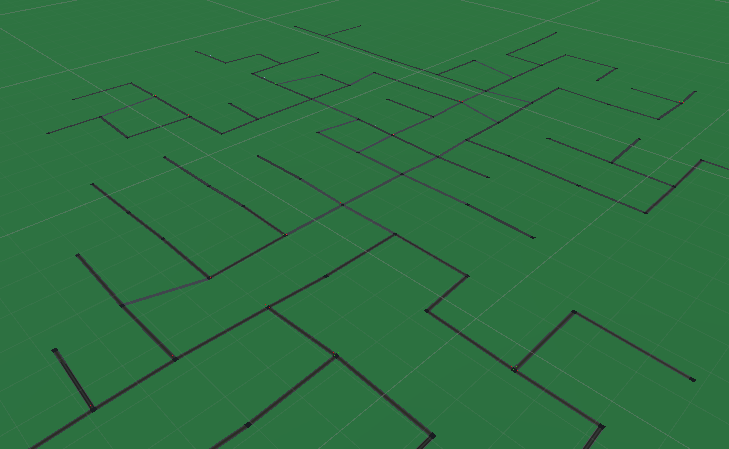
\includegraphics[width=\linewidth]{unitygraph.png}
\caption{Kép a generáló algoritmus eredményéről Unityben}
\label{fig:ugraph}
\end{figure}

\Chapter{Tervezés, implementáció}

- Bemutatni a használt eszközkészletet.
- UML osztálydiagram, szekvencia diagramok, blokkvázlat és hasonló dolgok.
- JavaScript implementációval kapcsolatos tudnivalók.
- WebGL-ről részletesen írni.

\Chapter{Szimulációk}

\Section{A szimuláció alakulása paraméterezés függvényében}
A paraméterezést az alkalmazáson belül megjelenő felületről lehet állítani. A következő értékek változtathatóak:
\begin{itemize}
\item{a közlekedési lámpák váltakozásainak ideje, másodpercben megadva},
\item{a szimulációban egyidőben maximálisan résztvevő autóbuszok száma},
\item{a szimulációban egyidőben maximálisan résztvevő személygépjárművek száma},
\item{két személygépjármű létrehozása közötti eltelt idő, másodpercben mérve},
\item{a város úthálózadának csomópontszáma},
\item{egy személygépjármű útjának maximális hossza, csomópontokban mérve}.
\end{itemize}
Ezen értékek közül a gráf csomópontszámán kívül mindegyik változtatható a város újra generálása nélkül. Az újra generálást egy \textit{Generate Anew} gombbal lehet elvégezni a felületen (\ref{fig:param}. ábra).
\begin{figure}[H]
\centering
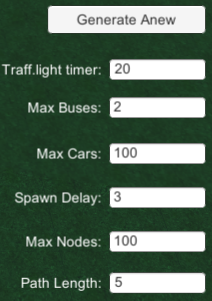
\includegraphics[scale=1.0]{params.png}
\caption{A paraméterek beállítási felülete, azok alapértelmezett értékeivel}
\label{fig:param}
\end{figure}

Az alapértelmezett paraméterekkel csekély forgalom jön létre egy kis méretű városban. Maga a város képe nagyjából tükrözi egy ilyen méretű város lehetséges elrendezését, az épületek típusai a központ felé bérházak, a peremeknél kertesházak. A szimuláció futása közben a kamerát a W,A,S,D gombokkal lehet mozgatni, valamint az egér görgőjével közelíteni és távolítani.

\subsection{Forgalmi szituációk}
A közlekedési szabályok is megfigyelhetőek az adott objektumoknál, az alábbi képeken ezt szemléltetem.
\begin{figure}[H]
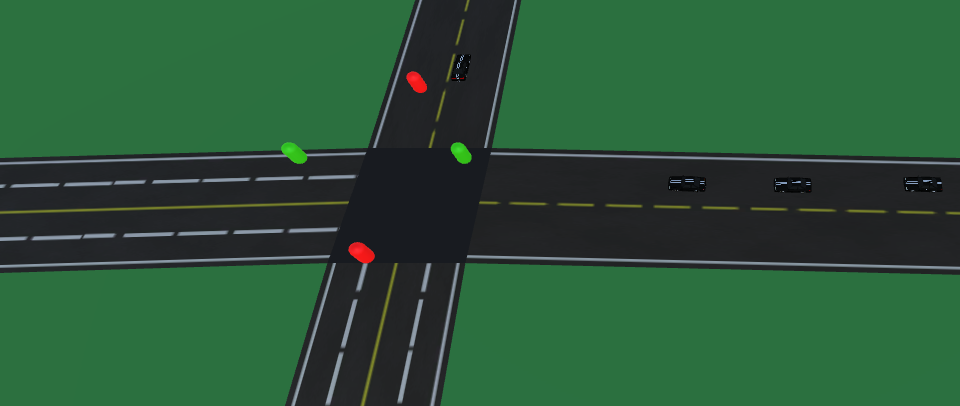
\includegraphics[width=\linewidth]{trafficLight.png}
\caption{Útkereszteződésnél várakozó autók éppen elindulnak}
\label{fig:xroadlight}
\end{figure}
\begin{figure}[H]
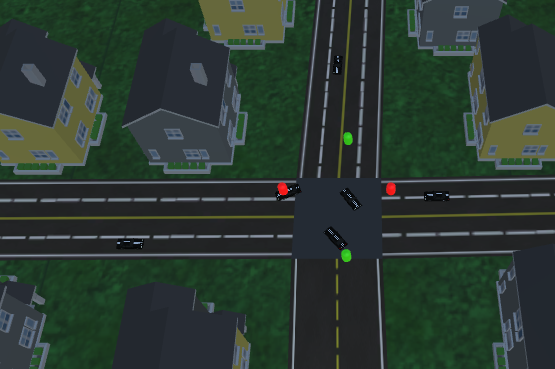
\includegraphics[width=\linewidth]{smalltowntraffic.png}
\caption{Többsávos úton a felülről párhuzamosan érkező autók balra és jobbra kanyarodnak, velük egyidőben szemben jövő autó pedig balra}
\label{fig:multilane}
\end{figure}
\begin{figure}[H]
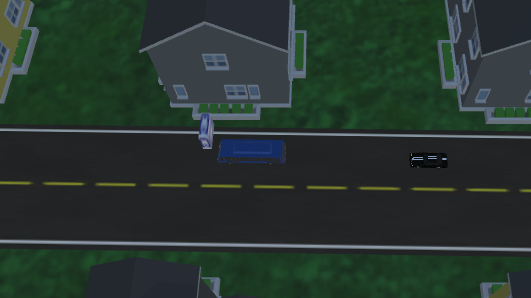
\includegraphics[width=\linewidth]{carwaiting.png}
\caption{Autó az előtte lévő autóbusz elindulását várja}
\label{fig:waiting}
\end{figure}
\begin{figure}[H]
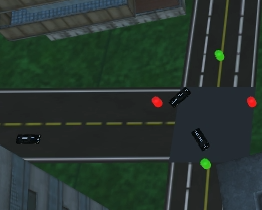
\includegraphics[width=\linewidth]{rofway.png}
\caption{Balra nagy ívben kanyarodó autó elengedi maga előtt a jobbra kis ívben kanyarodót}
\label{fig:rightofway}
\end{figure}

\subsection{Úthálózat mérete}
A generálás méretét tekintve nagyobb városoknál is elvártan működik. A legnagyobb méret amivel teszteltem, az egy 2000 csomópontból álló város. Ezt körülbelül 3 másodperc alatt generálja le egy átlagos számítógépen.
\begin{figure}[H]
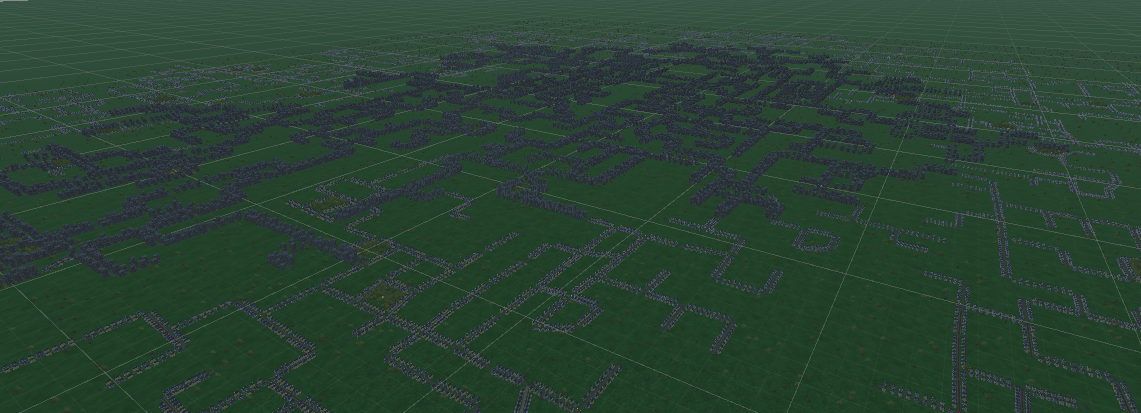
\includegraphics[width=\linewidth]{verybig.png}
\caption{Egy kétezer csomópontból álló város képe}
\label{fig:verybigcity}
\end{figure}

Kipróbáltam valamint egy kisebb, 10 csomópontból álló községet is, megjelenésében és funkcionalitásában ez is megfelelő.
\begin{figure}[H]
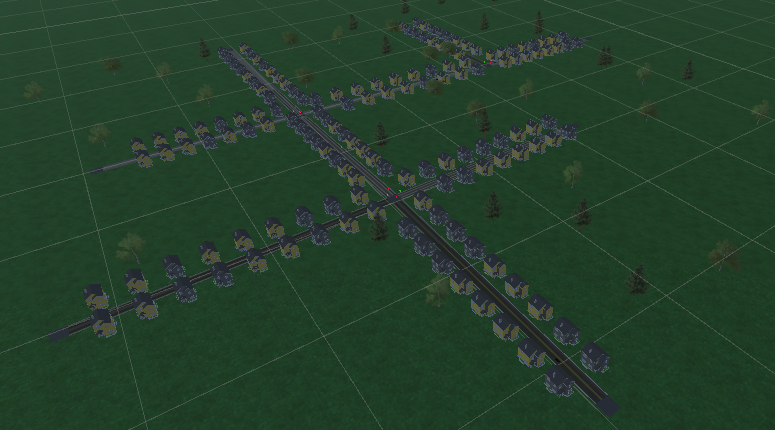
\includegraphics[width=\linewidth]{village.png}
\caption{Tíz csomópontból álló község}
\label{fig:smalltown}
\end{figure}

\subsection{A forgalom sűrűsége az úthálózat méretének függvényében}
A minimális egy másodperces késleltetés miatt az autók létrehozását illetően könnyebbnek találtam a forgalom vizsgálatát egy kisebb, nagyjából 20 csomópontból álló úthálózaton.

Itt észrevehető hogy átlagos forgalom akkor kezd el kialakulni, ha a ötször annyi mennyiségű jármű van az utakon, mint amennyi csomópontból áll az úthálózat. Ez a paraméterezés még nem okoz forgalmi dugót.
A jelzőlámpák váltási idejét felnövelve 40 másodpercre minimális lassulás észlelhető, de ezt ellensúlyozza az, hogy kevesebbszer kell megállnia egy autónak, ha sokáig egyenesen halad.
\begin{figure}[H]
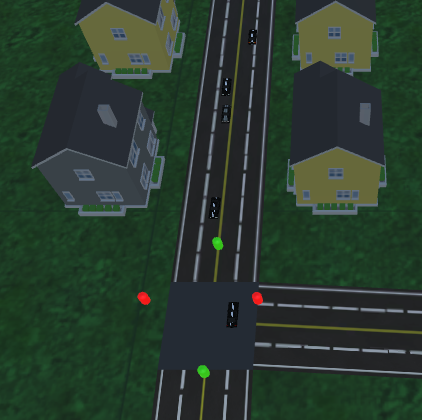
\includegraphics[width=\linewidth]{increasedtraffic.png}
\caption{Nemrég váltott jelzőlámpa előtt várakozik három autó (20 csomópont 100 autóval)}
\label{fig:trafficbigger}
\end{figure}

A parkok is viszonylag rendesen generálódnak, főleg a nagyobb méretű városokban figyelhető ez meg.
\begin{figure}[H]
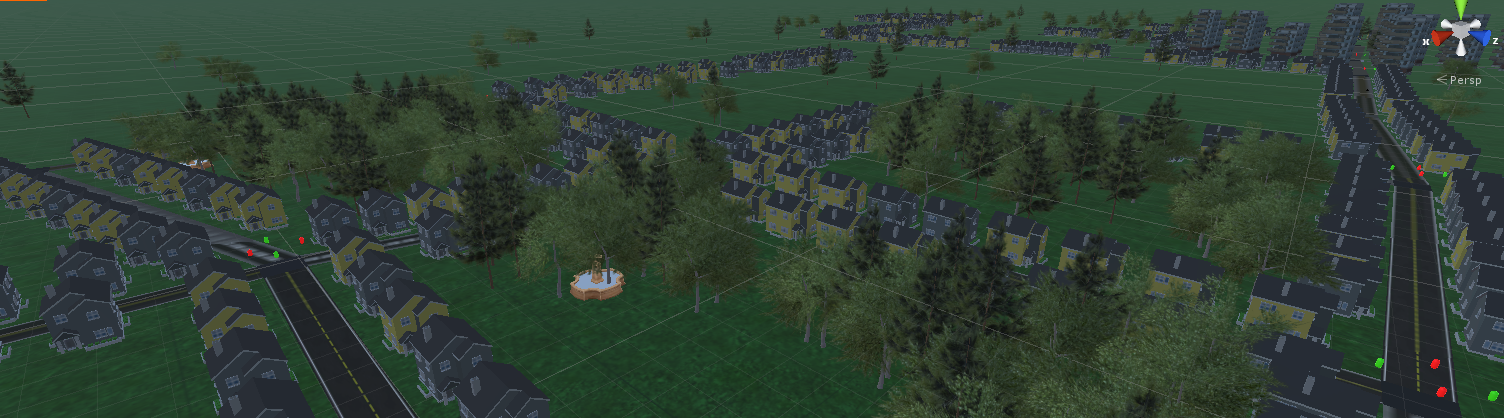
\includegraphics[width=\linewidth]{parks.png}
\caption{Parkok egymás mellett egy város szélén}
\label{fig:parks}
\end{figure}
\Chapter{Összegzés}

A feladat teljesítését természetesen az első részben leírt szoftverek vizsgálatával kezdtem, melyből megtudtam pár információt az ilyen jellegű szoftverek működéséről. Az ott leírtak összefoglalják, hogy egy átlagos ilyen célú szoftver milyen felépítéssel bír, általánosan milyen funkcióik vannak, valamint az általuk kezelt objektumok milyen tulajdonságokból épülnek fel.

A modell megalkotásánál definiált kritériumokat teljesítettem, az elkészült programban megjelennek az ott leírt elemek, forgalmi szituációk, azok működése a leírtak szerint történik.

A generálás folyamatát a harmadik részben dokumentáltam. Az algoritmus eredményéből látszik, hogy alkalmas a forgalmi helyzetek megjelenítésére, az átlagos közlekedésre. Városkép szempontjából elfogadható eredményt ad, az épületek és más díszítőelemek logikusan helyezkednek el a város területén.

A szimuláció tervezésével foglalkozó fejezetben részletesen dokumentáltam az egyes szkriptek működését, valamint a Unity Engine-en belüli implementációt. Az egyes algoritmusokat kódpéldákkal is szemléltettem. Szimuláció közben látható ennek az implementációnak az eredménye, a járművek mozgása a Unity fizikai motorján keresztül történik.

Az utolsó részben megvizsgáltam a paraméterezéssel kapcsolatban felállított követelmények teljesülését. A program a megalkotott felületen keresztül működésében befolyásolható, a különböző paraméterezések eredménye pedig szemmel látható.

Összefoglalva, a program feladatként kiírt célokat, bár közlekedésre vonatkozóan nem mélyül bele a rengeteg úthálózati elembe, való életben létező szabályokba, hanem ehelyett csak az egyszerű elemeket kezeli. Viszont a megalkotott szoftver nagyon könnyen bővíthető, a modellre építve egyszerűen lehet hozzáadni elemfajtákat ha az implementációt tekintjük.

% !TEX encoding = UTF-8 Unicode

\begin{thebibliography}{x}
\addcontentsline{toc}{chapter}{\bibname}

- https://www.researchgate.net/publication/228966705_A_Review_of_Traffic_Simulation_Software
- https://www.anylogic.com/road-traffic/

\end{thebibliography}


% !TEX encoding = UTF-8 Unicode
\newpage
\section*{CD-melléklet tartalma}

A dolgozat PDF változatát a \texttt{dolgozat.pdf} fájlban találjuk.

A dolgozat \LaTeX\ segítségével készült. A forrásfájlok a \texttt{dolgozat} jegyzékben találhatók.

\[
\ldots
\]



\end{document}
